\chapter[Analysis and identification of dysprosody]{Analysis and identification of dysprosody}
\label{ch4}

\section{State of knowledge}
\label{ch4_1}

The prosodic features of speech describe its stress and rhythm, speech to pause ratio and velocity, speech intensity and pitch variation \cite{Darley1975, Ackermann1997}. Prosody is an~important aspect of human verbal communication as it conveys semantic, syntactic and affective information and reflects emotions of a~speaker. Due to vocal tract muscle stiffness~\cite{Skodda2009} patients with PD exhibit alterations of rhythm and speech rate (inappropriate silences, short rushes of speech, and variable speech rate)~\cite{Brin2009}, small variations in pitch and intensity (monopitch and monoloudness, respectively)~\cite{Hart1990, Duffy2013} resulting into flat voice and speech melody lacking intonation \cite{Canter1963, Darley1975}. Such deterioration of prosody has a~detrimental impact on speech naturalness and intelligibility, and can ultimately lead to substantial voice and speech quality deficits resulting into serious day-to-day communication problems in patients suffering from PD.

\subsection{Monopitch}
\label{ch4_1_1}

In $2011$, based on their previously published research~\cite{Skodda2008}, authors Skodda et al.~\cite{Skodda2011b} analysed variability of pitch during a~reading task in a~sample of $138$ PD patients and $50$ healthy controls (HC), and showed significantly reduced pitch variability in PD patients in comparison with HC when related to the entire reading task confirming the results of the previous research in this area \cite{Metter1986, Flint1992, Goberman2005d}. In the same year, Rusz et al.~\cite{Rusz2011} demonstrated that even in the early stages of PD, patients do exhibit lower melody and decreased intensity variations referring to limited range of motions and impaired laryngeal tension in combination with insufficient breath support~\cite{Pinto2004}. Results of this study indicated that patients in the early stage of PD can suffer primarily from prosodic impairment, which is in accordance with the findings of Harel et al.~\cite{Harel2004b} stating that poor intonation had been observed in several individuals years before the onset of cardinal parkinsonian motor symptoms. Moreover, in their another study~\cite{Rusz2011}, Rusz et al. reported that reduced melody variations can be related to the lowered ability of stress pronunciation and emotional intonation limitation caused by the presence of HD. In $2014$, Tykalova et al.~\cite{Tykalova2014} investigated contrastive stress in $20$ male patients in early stage of PD and $16$ age- and gender-matched HC. The participants were asked to unnaturally emphasize several key words during a~reading task. In contrast with HC, PD patients produced a~distinctively flatter pitch contours, especially at the beginning and the end of a~phrase, confirming the findings published in \cite{Rusz2011, Rusz2011b}. In addition, Pell et al.~\cite{Pell2006} investigated impact of dysprosody on vocal-prosodic communication from the perspective of listeners and reported that listeners experienced serious difficulties recognizing the emotional prosody, sentence mode, phonemic stress and contrastive stress of PD patients compared to HC. And finally, in $2015$, Anand and Stepp~\cite{Anand2015} demonstrated that pitch variation is strongly correlated with the naturalness of speech perceived by listeners.

\subsection{Monoloudness}
\label{ch4_1_2}

In $1986$, authors Metter and Hanson proposed a~study in which they showed that patients with PD produced a~significantly smaller intensity variation compared to HC during the reading of a~standard passage~\cite{Metter1986}. Later, according to Watson and Munson, PD speakers exhibit overall lower speech intensity, deficits in intensity range, and intensity variations during speech production~\cite{Watson2008}. In addition to that, in $2011$, Skodda et al. proposed a~gender-related study of dysprosody in PD~\cite{Skodda2011c} comprising $169$ PD patients and $64$ age-matched HC and reported a~reduction in speech intensity during a~reading task composed of $4$ sentences. In the same year, Rusz et al.~\cite{Rusz2011} showed that early-staged PD patients can exhibit a~decreased intensity variations in comparison with HC. And finally, in $2014$, authors Clark et al.~\cite{Clark2014} performed a~study focused on loudness perception in $17$ PD patients and $25$ HC and showed that patients with PD produced a~significantly different pattern with more restricted range of perception when compared to healthy individuals.

\subsection{Speech rate deficits}
\label{ch4_1_3}

In $1963$, Canter~\cite{Canter1965} found no differences in the number of pauses or mean pause duration between PD patients and HC during a~reading task. However, in $1986$, Metter et al.~\cite{Metter1986} did demonstrate the presence of such speech rate abnormalities in HD. More recently, in $2008$, Skodda and Schlegel~\cite{Skodda2008} investigated articulation rate and pause time during reading of $170$-syllabic text composed of $4$ complex sentences in a~cohort of $121$ PD patients and $70$ HC. They analysed the performance of acoustic measurements applied on the first and the last sentence in order to evaluate the hypothesis of altered speech rate and rhythm in patients with PD and confirmed an age-related reduction of articulation rate that was proposed by Weismer~\cite{Weismer1984} back in $1984$. Furthermore, a~gender specific patterns of speech rhythm was referred. However, neither gender-related differences between PD patients and HC in speech rate parameters (total speech rate, net speech rate), nor overall distinctions in speech rate between PD and HC were observed. Later, in $2009$, Skodda et al. performed a~longitudinal study~\cite{Skodda2009} reporting speech rate variation closely related to the progression of PD and confirmed the previous findings of Ho et al.~\cite{Ho1999a}, in which decisive impairment of speech fluency was found specifically in the more advanced stages of PD. Two years later, in $2011$, Skodda et al. investigated net speech rate of patients with PD during a~reading task and observed no significant distinctions of this measure between PD patients and HC~\cite{Skodda2011b}. In addition, they reported increased number of pauses per second during a~reading task in their another work from the same year~\cite{Skodda2011c}. And finally, in $2015$, authors Bandini et al.~\cite{Bandini2015} employed a~study evaluating patterns of dysprosody in $14$ male and $6$ female PD patients via a~fully automated tool and showed that PD patients exhibit longer pauses between sentence repetitions. In contrast to the findings reported by Bandini et al., Skodda and colleagues performed several studies \cite{Skodda2010, Skodda2011c} reporting shorter pauses between sentences. However, as stated by Bandini et al. such distinction is a~consequence of a~difference between the speech tasks (sentence repetition task~\cite{Bandini2015} and reading of a~passage \cite{Skodda2010, Skodda2011c}).

\section{Rationale behind the research}
\label{ch4_2}

To summarize and emphasize, many researchers have performed studies focused on the investigation of a~variety of aspects associated with dysprosody in HD \cite{Canter1963, Metter1986, Caekebeke1991, Flint1992, Goberman2005b, Adams2009, Skodda2008, Rusz2011, Rusz2011b, Skodda2011c, Joan2015}. These studies comprised quantification, examination, and evaluation of intonation and melody of speech, variation in speech loudness and timing, contrastive stress and rhythmical deficits occurring with this disease. Regarding the monopitch aspect of HD, the literature have demonstrated that reduced variability in pitch is present in a~majority of patients suffering from PD. In the case of monoloudness aspect of HD, the presence of reduced variability in speech loudness in most patients with PD has been well-documented as well. Concerning speech rate disturbances associated with HD in PD, the previous studies do relate the rigidity and hypokinesia of the laryngopharyngeal tractus~\cite{Baker1998} and speech rate abnormalities~\cite{Skodda2009, Skodda2011b, Skodda2011c}. However, in contrast to the monopitch and monoloudness that seem to be describing dysprosody pretty well, the results on the speech rate in patients with PD still remains to be inconsistent~\cite{Caligiuri1989, Flint1992, Ackermann1997}.

This thesis builds upon the previous findings in this field of science, and proposes a~novel approach for accurate and sensitive identification of dysprosody in HD. So far, there is no work dealing with HD analysis and identification using a~poem recitation as well as a~comparison between neutral, stress-modified and rhymed speech. Introducing such speech tasks however is of scientific significance since the recitation task requires a~speaker to use precise and controlled variation in intonation and intensity of speech as well as speech rate/pausing all at once, and therefore this task is a~good candidate for sensitive differentiation of dysarthric and healthy speech. Next, the comparison between neutral, stressed, and rhymed speech is missing. However, it can provide useful information about distinctions in the patterns of prosodic impairments associated with HD when the speakers are exposed to a~variety of prosodic demands. Furthermore, most works that have been published does not perform the gender-differentiation, which in fact does neglect very important information that can provide deeper understanding of gender-specific patterns of dysprosody in HD. 

\section{Methodology}
\label{ch4_3}

\subsection{Description of the dataset}
\label{ch4_3_1}

For the purpose of this study, $149$ Czech native speakers were examined: $98$ patients with idiopathic PD ($59$ males and $39$ females, characteristics described as mean (sd): participants' age in years $67.52$ ($8.29$); duration of the disease in years $7.80$ ($4.42$); UPDRS~III (evaluation of motor functions)~\cite{Fahn1987} $24.91$ ($11.97$); UPDRS~IV (evaluation of complications of therapy; Hoehn and Yahr scale, staging of severity of PD)~\cite{Fahn1987} $2.83$ ($2.57$); RBDSQ (evaluation of sleep disorders)~\cite{Stiasny2007} $3.79$ ($3.23$); FOG-Q (evaluation of freezing of gait)~\cite{Giladi2000} $7.16$ ($5.81$); NMSS (evaluation of non-motor deficits)~\cite{Chaudhuri2007} $34.76$ ($19.80$); BDI (evaluation of depression) \cite{Beck2000, Beck1961} $13.19$ ($14.57$); MMSE (evaluation of cognitive dysfunctions)~\cite{Folstein1975} $28.07$ ($2.23$); LED (daily levodopa equivalent dose; in mg/day)~\cite{Lee2010} $1005.93$ ($545.66$)), and $51$ healthy speakers ($25$ males and $26$ females, characteristics described as mean (sd) as well: participant's age in years\footnote{Other clinical characteristics such as the scores of the clinical rating scales used to examine PD patients are not known for healthy speakers. For the purpose of this study, only patients with clinically diagnosed PD were further examined. So, age and gender of the participants are the only data available for healthy speakers.} $63.96$ ($9.21$)). For more information about demographical and clinical characteristics of the used cohort, especially for the group of male and female participants, see Table~\ref{tab:ch4_clinical_data}. 

All the speakers participating in this study were enrolled at the First Department of Neurology, St. Anne's University Hospital in Brno, Czech Republic. The healthy speakers had no history or presence of speech disorders or brain diseases, including neurological and psychiatric illnesses. All PD patients were examined on their regular dopaminergic medication approximately $1$~hour after the L-dopa~\cite{Lee2010} dose (i.\,e. ON state examination).

\begin{figure}[htb!]
	\centering
	\scriptsize
	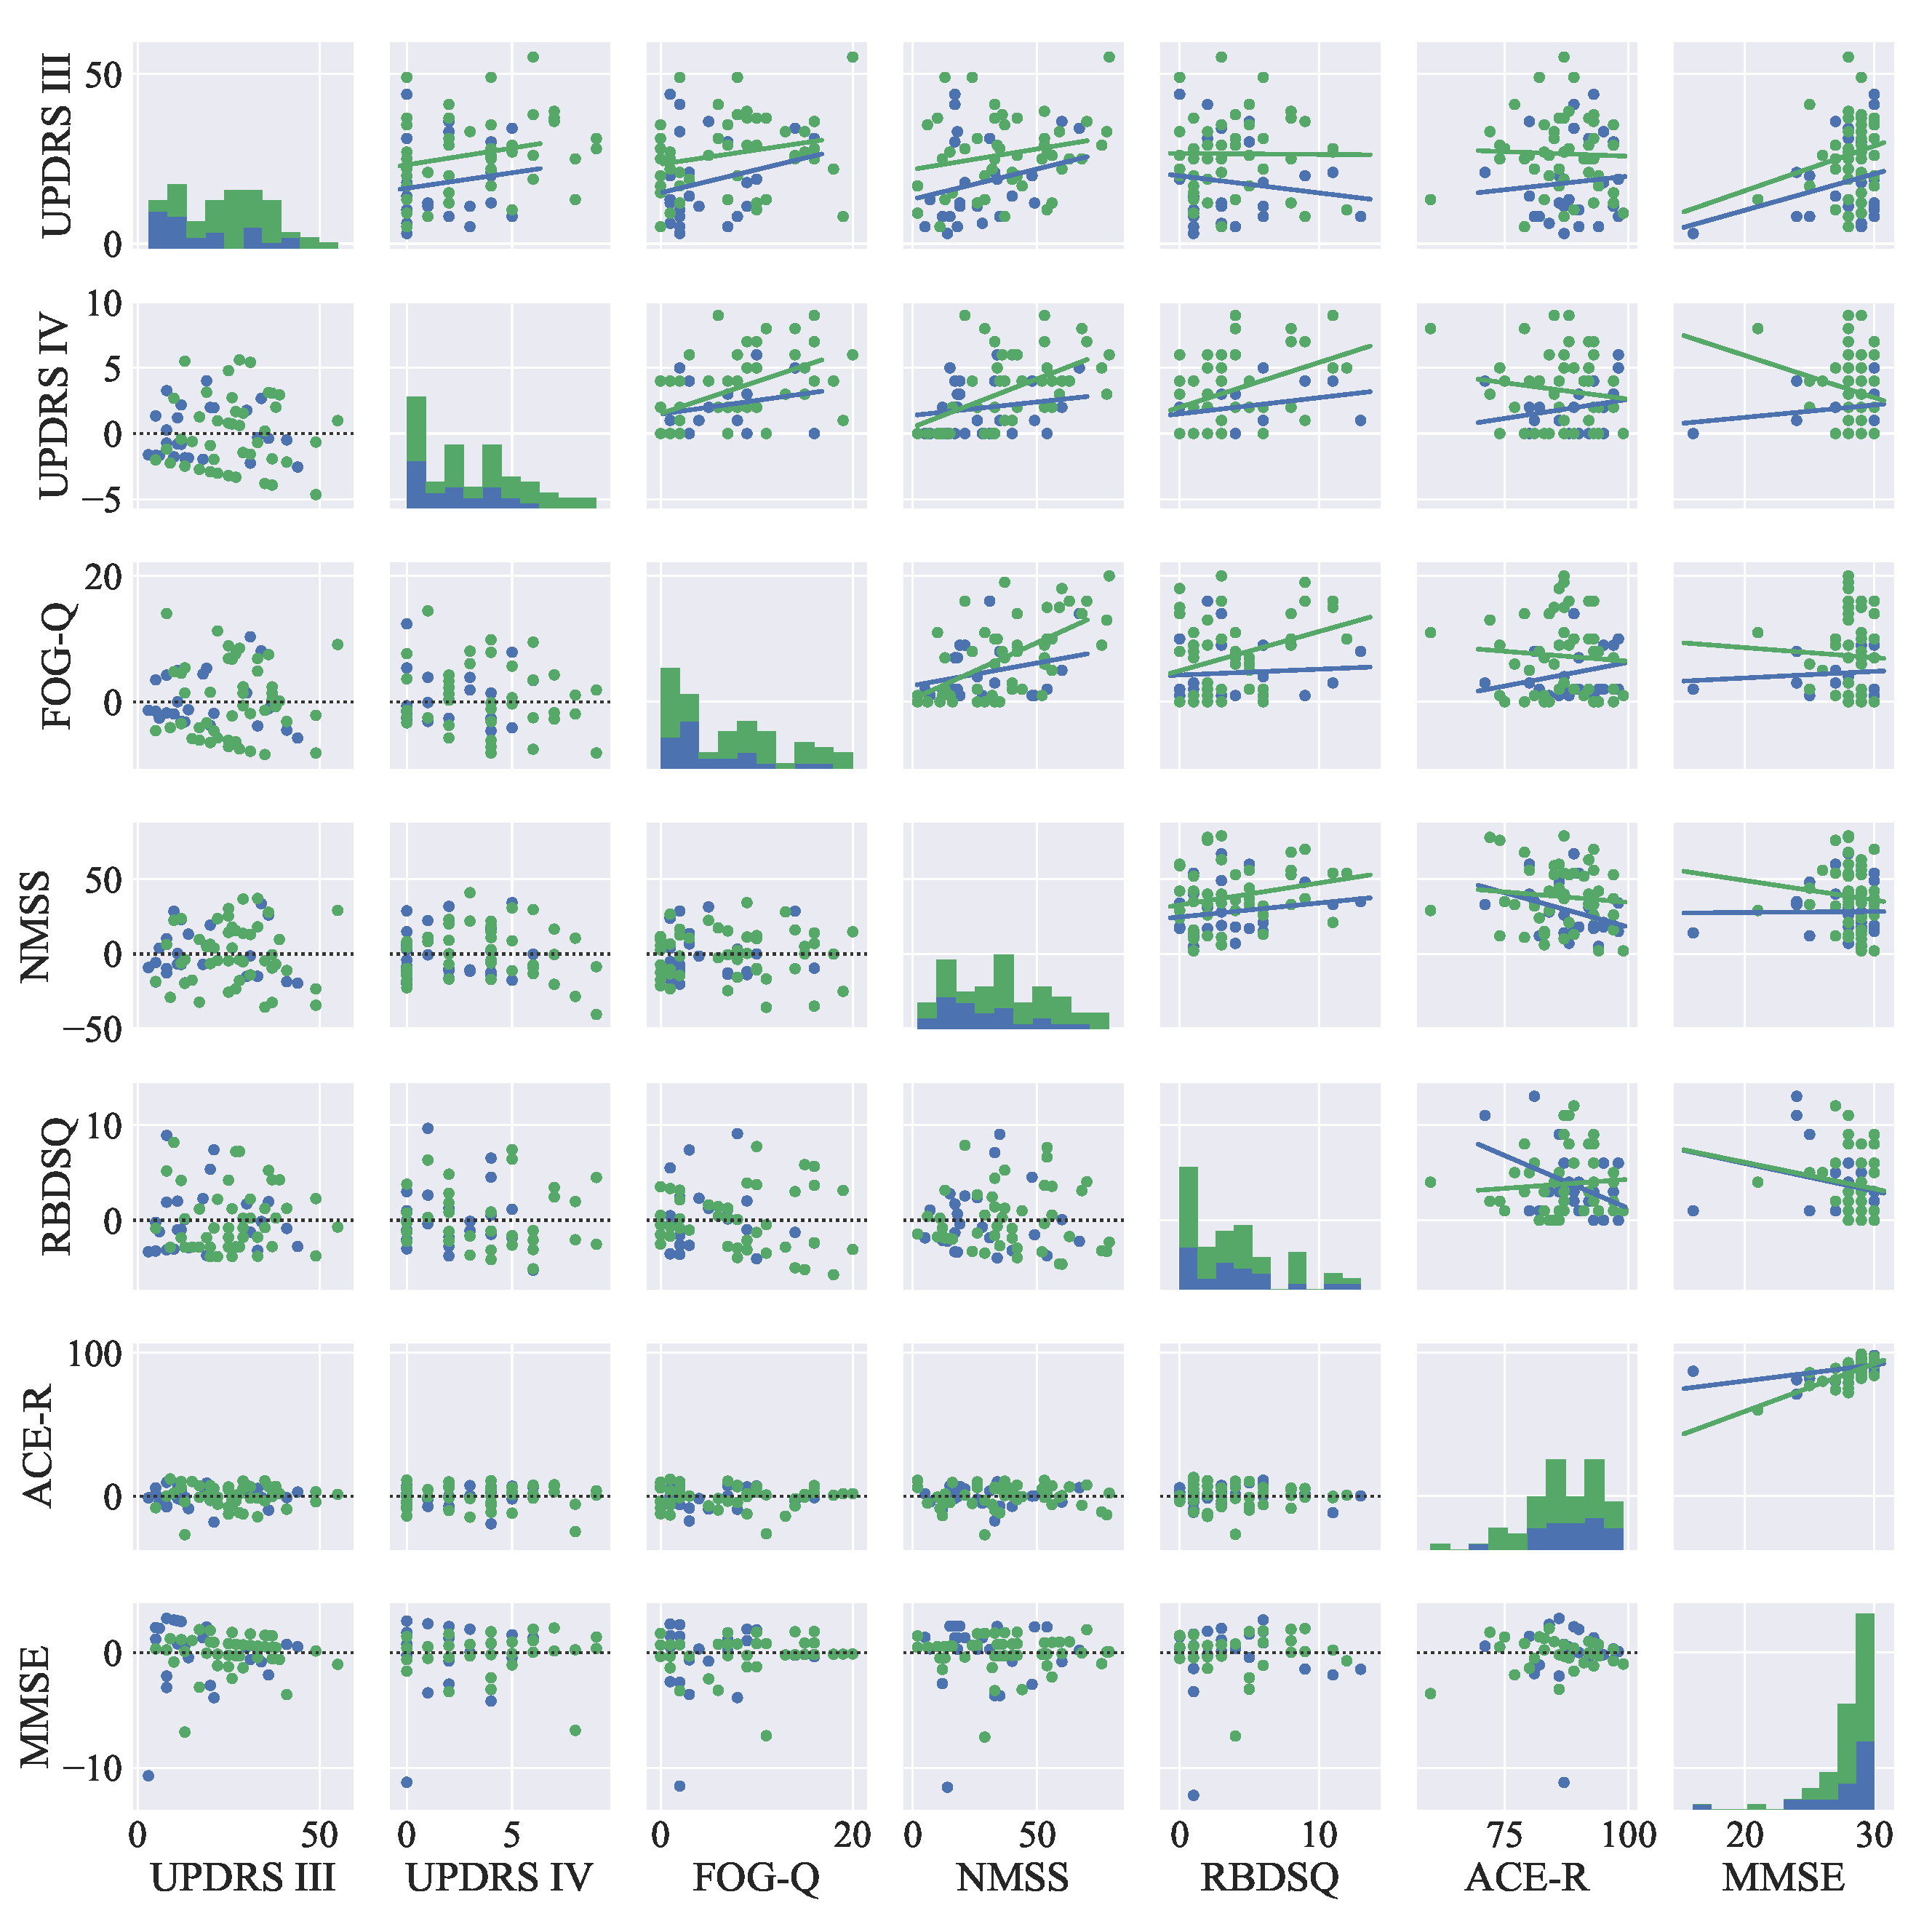
\includegraphics[width=0.99\textwidth]{pictures/ch4_clinical_statistics.eps}
	\caption[Descriptive statistical graphs of clinical data for PD patients.]{Descriptive statistical graphs of clinical characteristics (clinical rating scales) of PD patients participated in this study: on the main diagonal, histograms are visualized. Next, the upper triangular part of the graph-grid shows scatter plots along with the fitted lines of the robust linear regression models. And finally, the lower triangular part of the graph-grid is used to display residuals for the models shown in the the upper grid. Colour notation: blue colour represents female speakers, and green colour represents male speakers. For the description of the rating scales, see Table~\ref{tab:ch4_clinical_data}.}
	\label{fig:ch4_clinical_statistics}
\end{figure}

\begin{table*}[htb!]
	\centering
	\begin{threeparttable}
		\caption{Demographic and clinical characteristics of the participants.}
		\label{tab:ch4_clinical_data}
		\footnotesize
		\centering
		
		\begin{tabular}{l c c c c}
			\hline\hline\noalign{\smallskip}
			\rowcolor{gray_table}
			characteristics & PD (females) & PD (males) & HC (females) & HC (males) \\
			\noalign{\smallskip}\hline\noalign{\smallskip}

			Number of speakers  &           44         &           53         &           22         &           29         \\
			Age (years)         &   68.48~$\pm$~7.64   &   66.21~$\pm$~8.78   &   62.25~$\pm$~9.83   &   65.40~$\pm$~9.04   \\
			PD duration (years) &    7.61~$\pm$~4.85   &    7.83~$\pm$~4.39   &           -          &           -          \\
			UPDRS III           &   22.06~$\pm$~13.73  &   26.85~$\pm$~10.22  &           -          &           -          \\
			UPDRS IV            &    2.72~$\pm$~3.01   &    3.15~$\pm$~2.59   &           -          &           -          \\
			RBDSQ               &    3.42~$\pm$~3.48   &    3.85~$\pm$~2.99   &           -          &           -          \\
			FOG                 &    6.94~$\pm$~5.72   &    6.67~$\pm$~5.57   &           -          &           -          \\
			NMS                 &   36.03~$\pm$~26.72  &   38.19~$\pm$~19.72  &           -          &           -          \\
			BDI                 &   18.57~$\pm$~23.94  &    9.69~$\pm$~6.23   &           -          &           -          \\
			MMSE                &   27.38~$\pm$~3.63   &   28.56~$\pm$~1.05   &           -          &           -          \\
			LED (mg/day)        &  862.44~$\pm$~508.30 & 1087.00~$\pm$~557.47 &           -          &           -          \\
			
			\noalign{\smallskip}\hline\hline
		\end{tabular}
		
		\begin{tablenotes}
			\scriptsize
			\item Table notation: UPDRS~III\,--\,Unified Parkinson's disease rating scale, part~III: evaluation of motor function~\cite{Fahn1987}; UPDRS~IV\,--\,Unified Parkinson's disease rating scale, part~IV: evaluation of complications of therapy (Hoehn and Yahr scale, staging of severity of Parkinson's disease)~\cite{Fahn1987}; RBDSQ\,--\,The REM sleep behavior disorder screening questionnaire~\cite{Stiasny2007}; FOG-Q\,--\,Freezing of gait questionnaire~\cite{Giladi2000}; NMSS\,--\,Non-motor symptoms scale~\cite{Chaudhuri2007}; BDI\,--\,Beck depression inventory \cite{Beck2000, Beck1961}; MMSE\,--\,Mini-mental state examination~\cite{Folstein1975}; LED\,--\,L-dopa equivalent daily dose (mg/day)~\cite{Lee2010}.
		\end{tablenotes}
	\end{threeparttable}
\end{table*}

In addition to that, descriptive statistical graphs of specifically selected set of clinical characteristics for female and male speakers (only in the case of PD patients) can be seen in Figure~\ref{fig:ch4_clinical_statistics}. On the main diagonal, the graphs show histograms (i.\,e. approximation of a~distribution of the values of the clinical rating scales in the sample) for each of the rating scale. Next, on the upper triangular part of the graph-grid, scatter plots along with the lines fitted using robust linear regression can be seen. And finally, on the lower triangular part of the graph-grid, the residual plots for these models are visualized as well. With respect to the colour notation, blue colour represents female speakers and green colour represents male speakers.

Voice/speech signals were acquired by a~large capsule cardioid microphone M-AUDIO Nova~mounted to a~boom arm RODE PSA1. The microphone was positioned at a~distance of approximately $20$\,cm from the speaker's mouth. Room's environmental noise was lower than $30$\,dB sound pressure level. The signals were sampled with the sampling frequency of $48$\,kHz and consequently resampled to $16$\,kHz. All recordings were checked by a~trained acoustic engineer who discarded those, which contain some undesirable noise (such as speech therapist's cough, phone ringing, etc.). All the participants signed an informed consent form that had been approved by the Ethics Committee of St. Anne's University Hospital in Brno.

With respect to the speech tasks used to quantify prosodic deterioration in HD, the following three speech task scenarios comprising two reading tasks and a~poem recitation task were considered. First of all, every participant performed two reading tasks ($1$. emotionally-neutral reading, and $2$. stress-modified reading). Next, all speakers were asked to recite a~poem composed of two rhymes. At first, they were instructed to read the poem on a~paper. After that, every participant recited this poem into a~microphone, but without any need to keep it in memory (i.\,e. no memory-related constraints were applied). The tasks:
\begin{enumerate}

	\item Reading~a short paragraph with neutral emotion. 
	In Czech (original)\,--\,\textit{I na tom, \v{z}e \v{c}lov\v{e}k si opat\v{r}\'{i} psa, aby nebyl s\'{a}m, je mnoho pravdy. Pes opravdu nechce b\'{y}t s\'{a}m.}; In English\,--\,\textit{Even the fact that a~man gets a~dog to not be alone is pretty much true. A~dog really don't want to be alone.}

	\item Stress-modified reading. 
	In Czech (original)\,--\,\textit{Te\v{d} mus\'{i}\v{s} b\'{y}t chv\'{i}li trp\v{e}liv\'{y}, ne\v{z} to dokon\v{c}\textbf{}me. U\v{z} m\v{e} to nebav\'{i}, dej mi u\v{z} kone\v{c}n\v{e} pokoj! Tak co, jak to dopadlo?}; In English\,--\,\textit{Now, you have to be patient until we finish it. I'm tired of it already, leave me alone! So, how did it go?}

	\item Poem recitation task. 
	In Czech (original)\,--\,\textit{Chcete vid\v{e}t velk\'{y} lov? Budu lovit v d\v{z}ungli slov. Osedl\'{a}m si Pegasa, chyt\'{\i}m b\'{a}se\v{n} do lasa!}, ; In English\,--\,\textit{Would you like to see a~big hunt? I will be hunting in a~jungle of words. I will saddle the Pegasus, I will catch a~poem into a~lasso.}
\end{enumerate}

\subsection{Feature extraction}
\label{ch4_3_2}

To describe dysprosody in HD, several conventional and clinically well-interpretable acoustic features~\cite{Brabenec2017} were used. The following acoustic features quantifying a~relative variability of speech intonation were computed: standard deviation of F0\footnote{In the case of pitch variation, fundamental frequency (F0) was used~\cite{Boersma2012}.} (FOSD); relative standard deviation\footnote{Standard deviation divided by the mean of the variable.} of F0 (relF0SD); variation range\footnote{Difference between minimum and maximum value of the variable.} of F0 (FOVR); and relative variation range\footnote{Variation range divided by the mean of the variable.} of F0 (relF0VR). In the case of intensity variation, squared energy operator (SEO) and Teager-Kaiser energy operator (TEO) were computed to quantify the intensity of voice/speech signals. The following acoustic features quantifying a~relative variability of speech intensity were computed: standard deviation of SEO/TEO (SEOSD/TEOSD); relative standard deviation of SEO/TEO (relSEOSD/relTEOSD); variation range of SEO/TEO (SEOVR/TEOVR); and relative variation range of SEO/TEO (relSEOVR/relTEOVR). Next, several features describing speech rate and pausing abnormalities in HD, such as total speech time (TST), net speech time (NST), total pause time (TPT), total speech rate (TSR), net speech rate (NSR), total pause time (pauses longer than $50$\,ms) (TPT\,($50$\,ms)), articulation rate (AR), and speech index of rhythmicity (SPIR) were computed. For more information about these features, see Appendix~\ref{tab:prosodic_features}, and the review article focused on the acoustic analysis in patients with PD~\cite{Brabenec2017}.

\subsection{Analytical setup}
\label{ch4_3_3}

To obtain an insight into the statistical properties of the acoustic features used to quantify dysprosody in HD, the approach of Tsanas et al.~\cite{Tsanas2010} using Spearman's correlation coefficient ($\rho$) and mutual information (MI) between the features and the associated clinical diagnosis (HC/PD) was followed. Spearman's correlation coefficient is a~statistical measure of the strength of a~monotonic relationship between feature vectors and the associated response variable~\cite{Sheskin2007}. Mutual information is a~measure of the amount of the information shared by two random variables (the larger the value of MI, the stronger statistical association between feature and the response can be observed). MI is defined as follows:
\begin{equation}
	I(X; Y) = \int_X\int_Y f(x, y) \log_2 \left(\frac{f(x, y)}{f_X(x)f_Y(y)} \right),
\end{equation}
where $X$ and $Y$ are both random variables with the associated joint probability density function $f(x, y)$, and marginal density functions $f_X(x)$ and $f_Y(y)$, respectively. For the purpose of this study, marginal entropies $H(X)$ and $H(Y)$, and joint entropy $H(X,Y)$ were used to compute MI. With this approach, MI is defined as:
\begin{equation}
	I(X; Y) = H(X) + H(Y) - H(X, Y).
\end{equation}

Moreover, Mann-Whitney U~test was used to compare the distribution of the prosodic features between HC and patients with PD. The Mann-Whitney U~test is a~non-parametric statistical test that is used to assess whether two independent groups of variables are significantly different from each other~\cite{Birnbaum1956}. It is defined as:
\begin{equation}
	U = R_1 - \frac{n_1 (n_1 + 1)}{2},
\end{equation}
where $n_1$ is the sample size for sample $1$, and $R_1$ is the sum of the ranks in sample $1$. Note that it is not specified which sample is considered sample $1$, and therefore and equally valid statement can be made using sample $2$ ($n_2$ instead of $n_1$ and $R_2$ instead of $R_1$, respectively).

To evaluate an individual power of each of the acoustic features to discriminate healthy and dysarthric speech, every feature was used separately as an input to the random forest (RF) classifier (univariate models). Random forest is an ensemble learning algorithm operating by constructing a~multiple of base learners~\cite{Breiman2001} that are used for classifying new samples via voting mechanism. To optimise the trained models, grid-search technique over the set of tunable parameters was performed: the number of features over which RF performs a~search while constructing each branch was selected to be equal to the square root of the number of input features; and the maximum number of $500$ trees was chosen for this classifier.

Next, to build models capable of HD discrimination based on the combination of acoustic features, i.\,e. combination of the prosodic impairments present in HD, multivariate models were trained as well. For this purpose, RF classifier with the same tuning parameters as in the case of univariate models was used. However, to select only the relevant set of features and to build clinically interpretable models with low dimensionality (prediction models with less features are in general less prone overfitting), a~feature selection process was applied~\cite{Guyon2006}. For this purpose, a~modified version of sequential floating forward selection (SFFS) algorithm proposed by Pohjalainen et al.~\cite{Pohjalainen2014} in $2014$ was used.

To quantify the classification performance of the models, Matthew's correlation coefficient~\cite{Matthews1975} (MCC) as a~reference performance measurement employed on unbalanced data sets~\cite{Jurman2012}, accuracy (ACC), sensitivity (SEN), and specificity (SPE)\footnote{In the frame of this study, ACC, SEN, and SPE are are expressed in $\%$, and therefore should be rather referred to as: $P_\mathrm{ACC}$, $P_\mathrm{SEN}$, $P_\mathrm{SPE}$ as the ACC, SEN, and SPE are expressed as rational numbers. However, for the simplicity and easier interpretability of the results, classical abbreviations (ACC, SEN, SPE) are used.} were computed. MCC was also used as a~ measure assessing the classification performance of the models during a~feature selection process. All metrics however are useful when used to describe properties of the build models (described bellow). The metrics are defined as:
\begin{eqnarray}
	\mathrm{MCC} &=& \frac{TP \times TN + FP \times FN}{\sqrt{N}}, \\
	\mathrm{ACC} &=& \frac{TP + TN}{M} \cdot 100\,[\%], \\
	\mathrm{SEN} &=& \frac{TP}{TP + FN} \cdot 100\,[\%], \\
	\mathrm{SPE} &=& \frac{TN}{TN + FP} \cdot 100\,[\%],
\end{eqnarray}
where the variables denote: $N = (TP + FP)(TP + FN)(TN + FP)(TN + FN)$, $M = TP + TN + FP + FN$. $TP$ (true positive) and $FP$ (false positive) represents the number of correctly identified PD subjects and a~number of subjects identified as PD, but being healthy. Similarly, $TN$ (true negative) and $FN$ (false negative) represent the total number of correctly identified healthy controls, and PD patients identified as HC. In the frame of this study, these classification metrics can be interpreted as: accuracy expresses the proportion of correctly identified PD patients as well as healthy subjects ($TP + TN$) out of all subjects ($TP + TN + FP + FN$), so that with higher accuracy, fewer miss-classifications are made; sensitivity expresses the proportion of participants correctly identified as having PD ($TP$) out of all patients with PD ($TP + FN$), so that with higher sensitivity, fewer actual cases of PD go undetected; and specificity expresses the proportion of participants correctly identified not as having PD ($TN$) out of all healthy subjects ($TN + FP$), so that with higher specificity, fewer healthy subjects are labelled as having PD.

The theoretical chance level of binary classification is $50$\,\%. This threshold is based on the assumption of infinite sample size, which does not hold in practice. The empirical chance level depends on the actual number of samples in the used dataset and therefore it is common to see the empirical chance level noticeably above the theoretical threshold for small datasets ($60$\% or even higher)~\cite{Combrisson2015}. As the sample size grows, the empirical chance level is getting closer to its theoretical value. With the growing dimension of feature space required sample size grows exponentially. So, to find out if the classification results were obtained by chance or by the actual relationship between the class labels and the data a~non-parametric statistical method: permutation test was used. Permutation test is commonly used tool in biostatistical research. It makes no particular assumptions about statistical properties of the samples except that the observations are independent and identically distributed under the null hypothesis, which makes it highly attractive~\cite{Phipson2010}. The main idea behind permutation tests used in classifier performance evaluation is the following: The null hypothesis is that the observations are independently and identically distributed (in other words, there is no relation between the class labels and the data). The alternative hypothesis is that the distribution differs between groups (in our case between PD and HC groups). The null hypothesis testing requires the p-value to be determined. The most commonly used approach is to estimate the p-value by randomly permuting the labels to obtain the empirical null distribution~\cite{Phipson2010}, however, in the frame of this study, the exact p-value is used to mitigate the type~I error rate and the multiple testing issues~\cite{Phipson2010}.

Thus, if the computed p-value is bellow a~chosen significance level $\alpha$ then the null hypothesis can be rejected. In this study, the $\alpha$ of $0.01$ was selected. Tested classification models with p-values bellow $\alpha$ were consider sufficiently high above chance level. Matthew's correlation coefficient was chosen as a~test statistic for the permutation test as it is the measure used to assess the classification performance of the models during a~feature selection step. The number of permutations was selected to be equal to $1000$ and the classifier validation was conducted using stratified $10$-fold cross-validation with $20$ repetitions~\cite{Ojala2009, Combrisson2015}.

\section{Results}
\label{ch4_4}

Results of the univariate analysis are summarized in Table~\ref{tab:ch4_statistical_analysis}. As can be seen, the best classification performance in terms of the classification accuracy computed for the univariate models can be summarized as follows: a) poem recitation task\,--\,$\mbox{ACC}=64.2\,\%$ (female participants), $\mbox{ACC}=64.6\,\%$ (male participants), and $\mbox{ACC}=68.5\,\%$ (all participants); b) reading with neutral emotion\,--\,$\mbox{ACC}=62.7\,\%$ (female participants), $\mbox{ACC}=69.1\,\%$ (male participants), and $\mbox{ACC}=58.4\,\%$ (all participants); and c) stress-modified reading\,--\,$\mbox{ACC}=68.7\,\%$ (female participants), $\mbox{ACC}=67.1\,\%$ (male participants), and $\mbox{ACC}=59.7\,\%$ (all participants).

\begin{table*}[tb!]
	\centering
	\begin{threeparttable}
		\caption{Statistical analysis of the prosodic features.}
		\label{tab:ch4_statistical_analysis}
		\footnotesize
		\centering
		\begin{tabular}{l l l r c c c c c} 
		
		\hline\hline\noalign{\smallskip}
		\rowcolor{gray_table}
		gender & features & disorder & $\rho$ & MI & $p$ & ACC & SEN & SPE \\
		\noalign{\smallskip}
		& \multicolumn{6}{c}{Poem recitation task} \\
		\noalign{\smallskip}\hline\noalign{\smallskip}

			\multirow{3}{*}{females}
			& relSEOSD & monoloudness &  0.10 & 0.97 &    & 64.2 & 72.5 & 51.9 \\
			& NST      & speech rate  & -0.23 & 0.88 &    & 62.7 & 67.5 & 55.6 \\
			& NSR      & speech rate  &  0.23 & 0.88 &    & 61.2 & 65.0 & 55.6 \\
			\noalign{\smallskip}

			\multirow{3}{*}{males}
			& F0VR     & monopitch    & -0.12 & 0.90 &    & 64.6 & 64.3 & 65.4 \\
			& TEOVR    & monoloudness & -0.18 & 0.90 &    & 62.2 & 62.5 & 61.5 \\
			& rellF0SD & monopitch    & -0.21 & 0.90 &    & 61.0 & 67.9 & 46.2 \\
			\noalign{\smallskip}

			\multirow{3}{*}{all} 
			& TPT & speech rate & -0.17 & 0.94 & *  & 68.5 & 70.8 & 64.2 \\
			& NST & speech rate & -0.11 & 0.79 &    & 63.1 & 69.8 & 50.9 \\
			& NSR & speech rate &  0.11 & 0.79 &    & 61.8 & 69.8 & 47.2 \\

		\noalign{\smallskip}\hline\noalign{\smallskip}
		& \multicolumn{6}{c}{Reading with neutral emotion} \\
		\noalign{\smallskip}\hline\noalign{\smallskip}
			
			\multirow{3}{*}{females}
			& F0VR          & monopitch   & -0.07 & 0.97 &    & 62.7 & 67.5 & 55.6 \\
			& TPT\,(50\,ms) & speech rate &  0.05 & 0.94 &    & 61.2 & 60.0 & 63.1 \\
			& AR            & speech rate & -0.05 & 0.94 &    & 61.2 & 60.0 & 63.0 \\
			\noalign{\smallskip}

			\multirow{3}{*}{males}
			& relSEOVR & monoloudness & -0.06 & 0.90 &    & 64.6 & 71.4 & 50.0 \\
			& relTEOSD & monoloudness &  0.27 & 0.90 & *  & 62.2 & 64.3 & 57.7 \\
			& relTEOVR & monoloudness &  0.28 & 0.90 & ** & 61.1 & 66.1 & 50.0 \\
			\noalign{\smallskip}

			\multirow{3}{*}{all}
			& relSEOSD      & monoloudness &  0.04 & 0.94 &    & 58.4 & 60.4 & 54.7 \\
			& relSEOVR      & monoloudness & -0.01 & 0.94 &    & 57.7 & 60.4 & 52.8 \\
			& TPT\,(50\,ms) & speech rate  &  0.03 & 0.82 &    & 54.4 & 58.3 & 47.2 \\
			
		\noalign{\smallskip}\hline\noalign{\smallskip}			
		& \multicolumn{6}{c}{Stress-modified reading task} \\
		\noalign{\smallskip}\hline\noalign{\smallskip}
			
			\multirow{3}{*}{females}
			& relTEOVR & monoloudness & -0.36 & 0.97 & ** & 68.7 & 70.0 & 66.7 \\
			& F0SD     & monopitch    & -0.22 & 0.97 &    & 64.2 & 65.0 & 63.0 \\
			& relTEOSD & monoloudness & -0.38 & 0.97 & ** & 59.7 & 55.0 & 66.7 \\
			\noalign{\smallskip}

			\multirow{3}{*}{males}
			& TPT\,(50\,ms) & speech rate  & -0.29 & 0.83 & *  & 67.1 & 71.4 & 57.7 \\
			& AR            & speech rate  &  0.29 & 0.83 & *  & 67.1 & 71.4 & 57.7 \\
			& relTEOVR      & monoloudness &  0.03 & 0.90 &    & 59.8 & 67.9 & 42.3 \\
			\noalign{\smallskip}

			\multirow{3}{*}{all}
			& TPT   & speech rate  & -0.26 & 0.93 & ** & 59.7 & 65.6 & 49.1 \\
			& F0SD  & monopitch    & -0.26 & 0.94 & ** & 57.8 & 61.5 & 51.0 \\
			& TEOVR & monoloudness & -0.15 & 0.94 &    & 57.7 & 62.5 & 49.1 \\
			
			\noalign{\smallskip}\hline\hline
		\end{tabular}
		
		\begin{tablenotes}
			\scriptsize
			\item Table notation: $\rho$\,--\,Spearman's rank correlation coefficient; MI\,--\,mutual information; $p$\,--\,p-values of Mann-Whitney U test (* means $p<0.05$; ** means $p<0.01$); ACC\,--\,classification accuracy; SEN\,--\,classification sensitivity; SPE\,--\,classification specificity. ACC, SEN, SPE: expressed in $\%$.
		\end{tablenotes}
	\end{threeparttable}
\end{table*}

Regarding the Mann-Whitney U~test, there are few statistically significant differences, specifically: a) poem recitation task\,--\,$p<0.01$ for TPT (all participants); b) reading with neutral emotion\,--\,$p<0.05$ for relTEOSD (males), and $p<0.01$ for relTEOVR (males); and c) stress-modified reading\,--\,$p<0.05$ for TPT\,(50\,ms) (males), AR (males), and $p<0.01$ for relTEOVR (females), relTEOSD (females), TPT (all participants), and F0SD (all participants). Next, a~comparison of the features expressing monopitch (F0SD), monoloudness (SEOSD), and speech rate abnormalities (NSR) between PD patients and HC can be seen in Table~\ref{tab:ch4_comparisons} and Figures~\ref{fig:ch4_comparisons_females},~\ref{fig:ch4_comparisons_males}, and~\ref{fig:ch4_comparisons_all}.

\begin{table}[!htb]
	\centering
	\begin{threeparttable}
		\caption{Comparison of acoustic features between PD speakers and HC.}
		\label{tab:ch4_comparisons}
		\footnotesize
		\centering
		\begin{tabular}{l l l c c c} 

			\hline\hline\noalign{\smallskip}
			\rowcolor{gray_table}
			gender & features & disorder & PD & HC & diff [\%] \\
			\noalign{\smallskip}
			\multicolumn{6}{c}{Poem recitation} \\
			\noalign{\smallskip}\hline\noalign{\smallskip}
			
			\multirow{3}{*}{females} &
			  F0SD  & monopitch    & 101.87~$\pm$~8.01 & 107.42~$\pm$~8.91 & PD < HC (5.17) \\
			& SEOSD & monoloudness &   6.30~$\pm$~3.67 &   5.61~$\pm$~3.17 & PD > HC (12.30) \\
			& NSR 	& speech rate  &  15.53~$\pm$~2.66 &  19.24~$\pm$~17.94 & PD < HC (19.28) \\
			\noalign{\smallskip}
			
			\multirow{3}{*}{males} &
			  F0SD  & monopitch    &  75.55~$\pm$~14.06 &  80.90~$\pm$~11.18 & PD < HC (6.61) \\
			& SEOSD & monoloudness &   6.44~$\pm$~3.48  &   7.02~$\pm$~3.67 & PD < HC (8.26) \\
			& NSR 	& speech rate  &  18.09~$\pm$~12.71 &  16.14~$\pm$~2.95 & PD > HC (17.10) \\
			\noalign{\smallskip}
			
			\multirow{3}{*}{all} &
			  F0SD  & monopitch    &  86.49~$\pm$~17.60 &  94.06~$\pm$~16.64 & PD < HC (8.05) \\
			& SEOSD & monoloudness &   6.42~$\pm$~3.54  &   6.28~$\pm$~3.48 & PD > HC (2.23) \\
			& NSR 	& speech rate  &  17.00~$\pm$~9.82  &  17.65~$\pm$~12.71 & PD < HC (3.68) \\
			
			\noalign{\smallskip}\hline\noalign{\smallskip}
			\multicolumn{6}{c}{Reading with neutral emotion} \\
			\noalign{\smallskip}\hline\noalign{\smallskip}				
			
			\multirow{3}{*}{females} &
			  F0SD  & monopitch    &  93.69~$\pm$~8.58  &  98.27~$\pm$~7.58 & PD < HC (4.66) \\
			& SEOSD & monoloudness &   5.97~$\pm$~3.37  &   6.03~$\pm$~2.67 & PD < HC (1.00) \\
			& NSR 	& speech rate  &  14.24~$\pm$~4.78  &  13.91~$\pm$~4.59 & PD > HC (2.37) \\
			\noalign{\smallskip}
			
			\multirow{3}{*}{males} &
			  F0SD  & monopitch    &  71.81~$\pm$~12.36 &  70.51~$\pm$~11.33 & PD > HC (1.84) \\
			& SEOSD & monoloudness &   6.67~$\pm$~3.03  &   5.42~$\pm$~2.15 & PD > HC (23.06) \\
			& NSR 	& speech rate  &  13.49~$\pm$~3.29  &  12.86~$\pm$~1.86 & PD > HC (4.90) \\
			\noalign{\smallskip}
			
			\multirow{3}{*}{all} &
			  F0SD  & monopitch    &  80.86~$\pm$~15.40 &  84.26~$\pm$~16.90 & PD < HC (4.04) \\
			& SEOSD & monoloudness &   6.39~$\pm$~3.16  &   5.68~$\pm$~2.42 & PD > HC (12.50) \\
			& NSR 	& speech rate  &  13.77~$\pm$~3.97  &  13.42~$\pm$~3.46 & PD > HC (2.61) \\
			
			\noalign{\smallskip}\hline\noalign{\smallskip}
			\multicolumn{6}{c}{Stress-modified reading} \\
			\noalign{\smallskip}\hline\noalign{\smallskip}

			\multirow{3}{*}{females} &
			  F0SD  & monopitch    &  91.27~$\pm$~11.13 &  95.72~$\pm$~6.71 & PD < HC (4.65) \\
			& SEOSD & monoloudness &   5.57~$\pm$~2.71  &   5.55~$\pm$~2.53 & PD > HC (0.36) \\
			& NSR 	& speech rate  &  17.20~$\pm$~3.22  &  19.44~$\pm$~12.40 & PD < HC (11.52) \\
			\noalign{\smallskip}

			\multirow{3}{*}{males} &
			  F0SD  & monopitch    &  68.87~$\pm$~10.11 &  74.86~$\pm$~13.44 & PD < HC (8.00) \\
			& SEOSD & monoloudness &   6.53~$\pm$~3.27  &   5.57~$\pm$~2.62 & PD > HC (17.24) \\
			& NSR 	& speech rate  &  19.35~$\pm$~8.95  &  18.37~$\pm$~4.45 & PD > HC (5.33) \\
			\noalign{\smallskip}
			
			\multirow{3}{*}{all} &
			  F0SD  & monopitch    &  78.05~$\pm$~15.42 &  85.50~$\pm$~14.44 & PD < HC (8.71) \\
			& SEOSD & monoloudness &   6.16~$\pm$~3.07  &   5.48~$\pm$~2.52 & PD > HC (12.41) \\
			& NSR 	& speech rate  &  18.49~$\pm$~7.15  &  18.82~$\pm$~9.17 & PD < HC (1.75) \\

			\noalign{\smallskip}\hline\hline
		\end{tabular}
		
		\begin{tablenotes}
			\scriptsize
			\item Table notation: diff [\%]\,--\,difference between the mean values for patients with PD and HC. All prosodic features for PD patients and HC are represented as mean~$\pm$~sd.
		\end{tablenotes}
	\end{threeparttable}
\end{table}

\newpage
From the perspective of the monopitch, reduced variation in F0 can be observed in $8$ out of the total number of $9$ scenarios. The only exception occurs in the case of male speakers reading a~passage with neutral emotion, which in general does not require that much variation in speech intonation or stress, so that this particular deviation is quiet acceptable. Regarding the monoloudness, interestingly there are $7$ cases in which PD patients show more variation in speech intensity than HC, which is in contradiction with the original assumption of lowered variation in speech intensity in patients with PD in comparison with HC. The only two exceptions lies in the neutral reading task, and the poem recitation task performed by male speakers. However, in contrast to that, female patients did show significantly lower speech intensity when compared to HC while performing the poem recitation. Thus, the results suggest a~presence of a~gender-related pattern of parkinsonian speech intensity variation and control deterioration. Finally, in the case of speech rate abnormalities, PD patients seem to have lower speech rate that HC when performing a~task that requires stress (stress-modified reading) or changes in the melody of speech (poem recitation). In the case of male participants, PD patients seem to have higher speech rate when compared to HC. And finally, in the case of female participants, the same phenomenon can be observed when the data for both genders are merged together.

\begin{figure}[htb!]
	\centering
	\scriptsize
	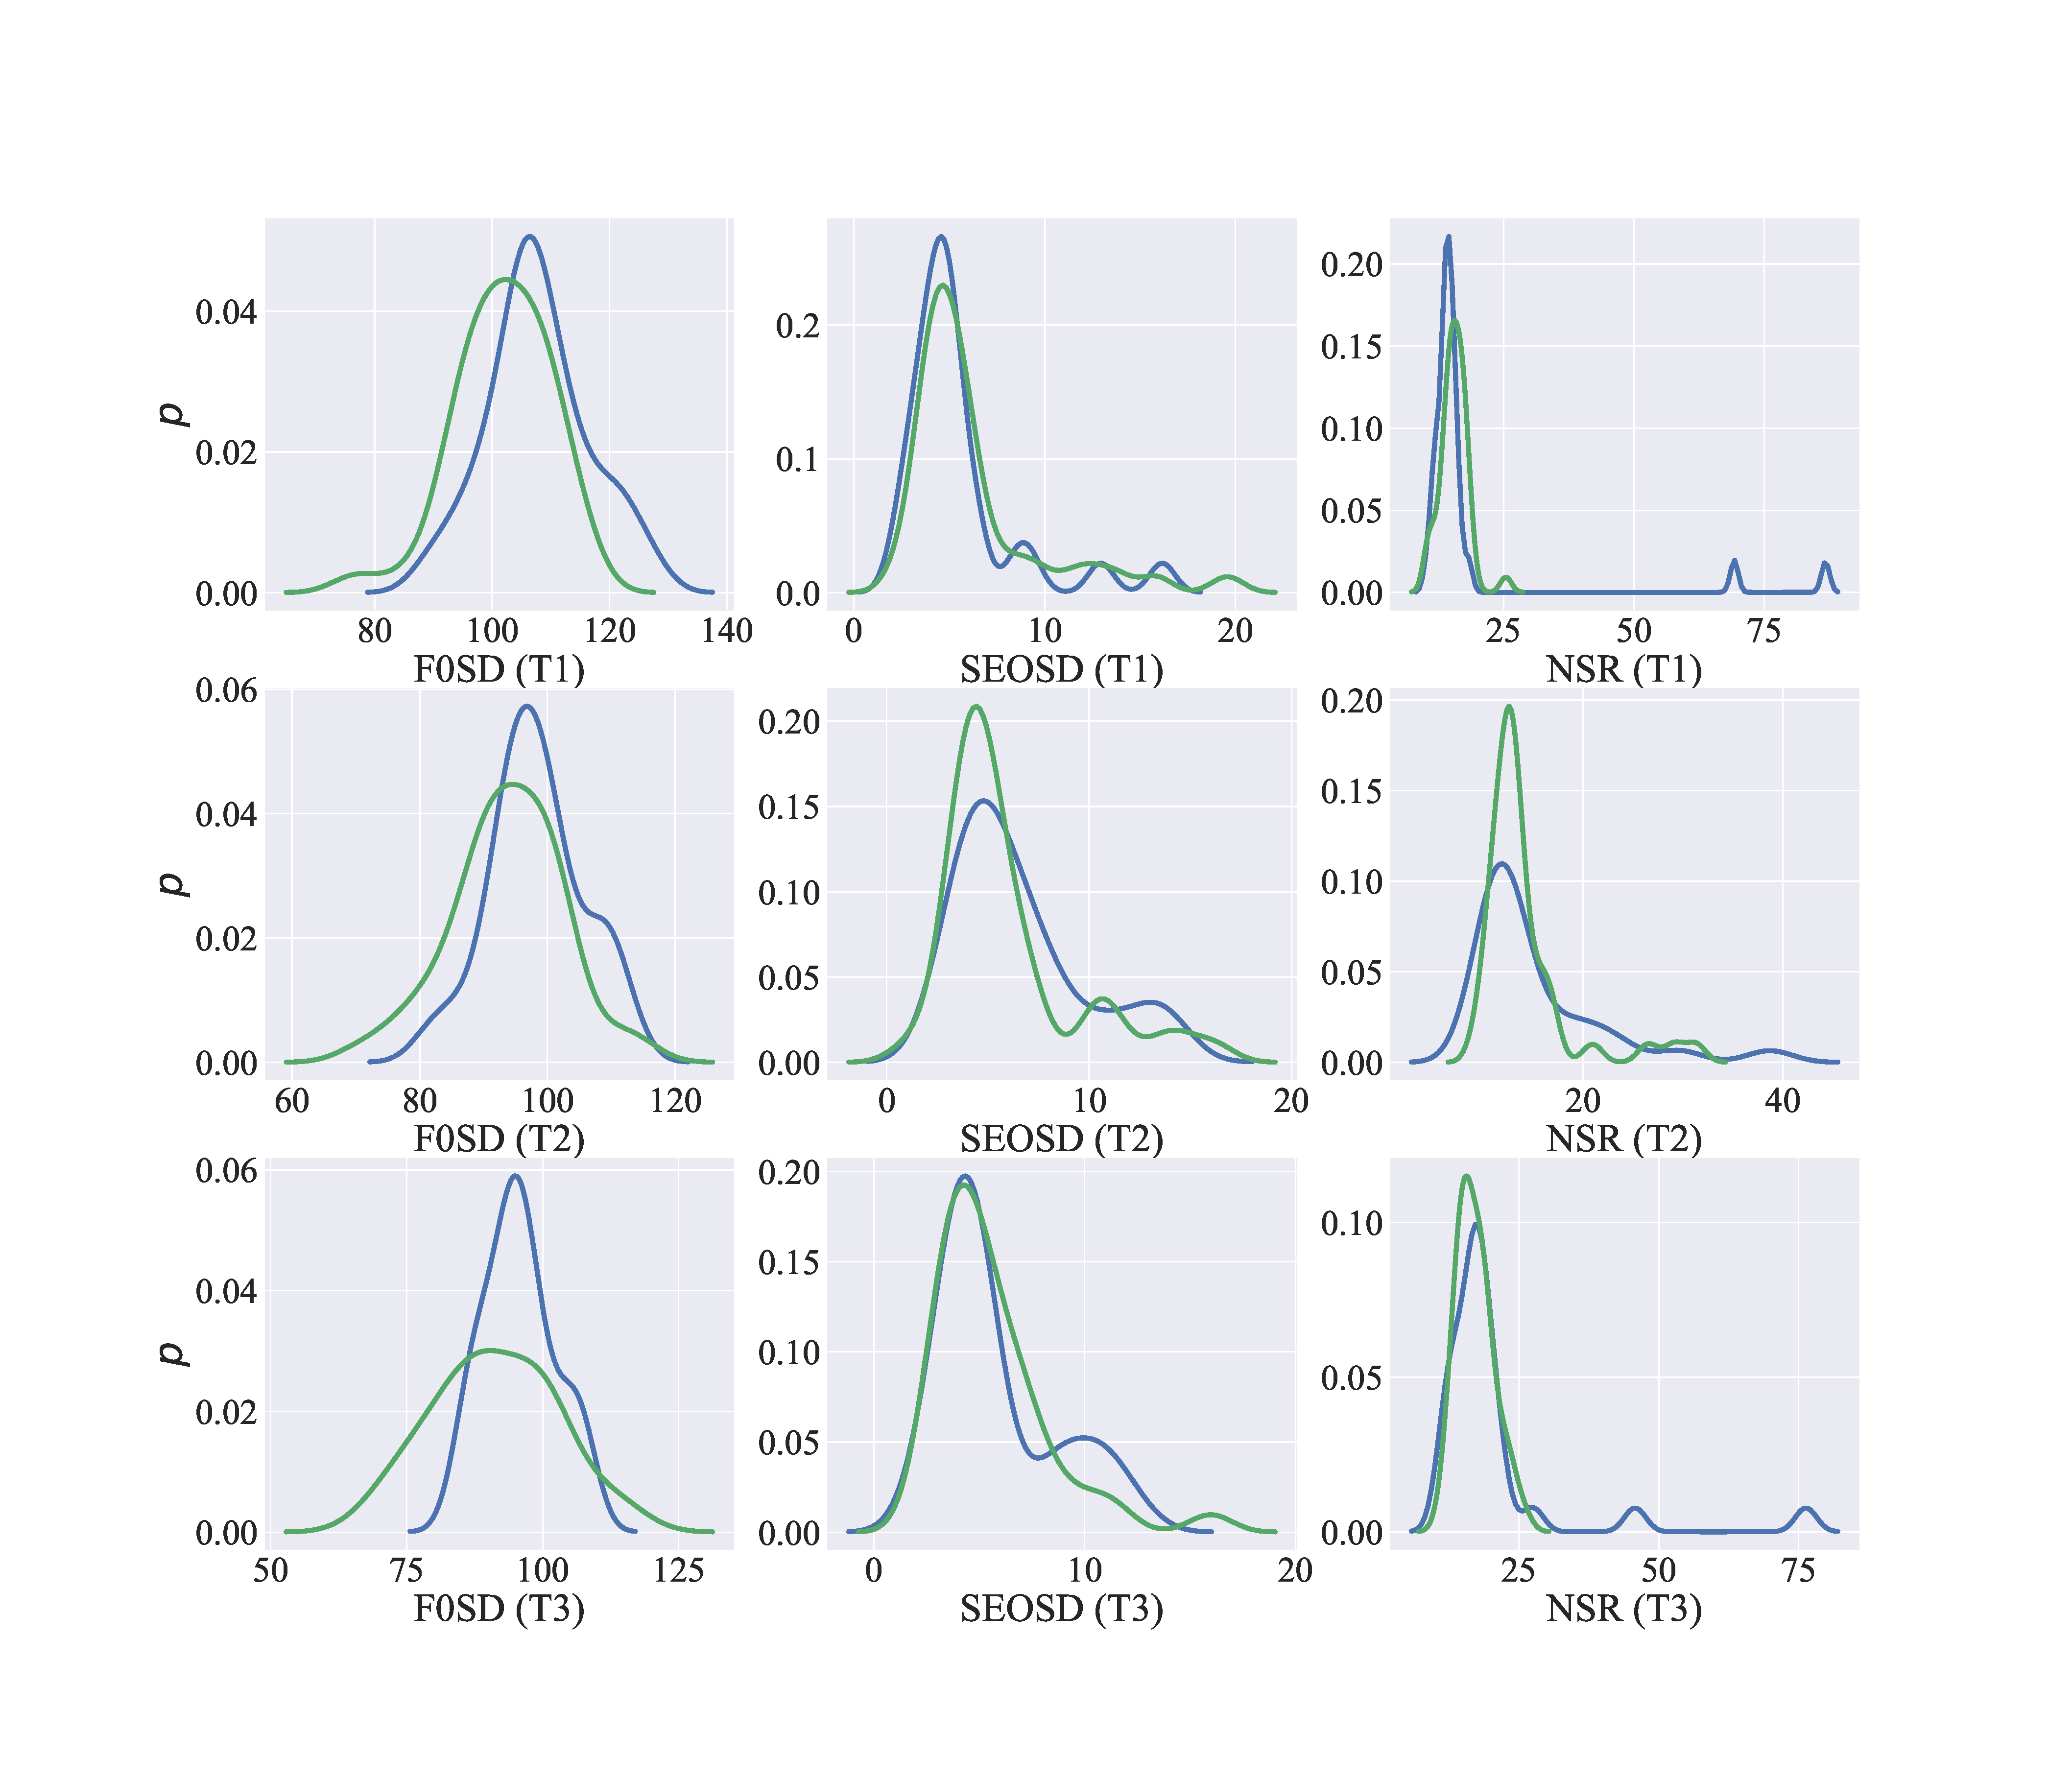
\includegraphics[width=0.99\textwidth]{pictures/ch4_comparisons_females.eps}
	\caption[Density estimation plots for female speakers.]{Density estimation plots (computed using kernel probability density estimation with Gaussian kernels) for selected acoustic features for all three speech tasks performed by female speakers only: T1\,--\,poem recitation task (first row); T2\,--\,emotionally-neutral reading (second row); and T3\,--\,stress-modified reading (third row). Colour notation: blue colour represents healthy speakers, and green colour represents speakers with PD. Feature notation: F0SD (standard deviation of fundamental frequency) expresses variability of intonation (melody of speech); SEOSD (standard deviation of squared energy operator) expresses variability of speech intensity (melody of speech); and NSR (net speech rate) expresses the number of phones per entire duration of speech without pauses (speech rate).}
	\label{fig:ch4_comparisons_females}
\end{figure}

\begin{figure}[htb!]
	\centering
	\scriptsize
	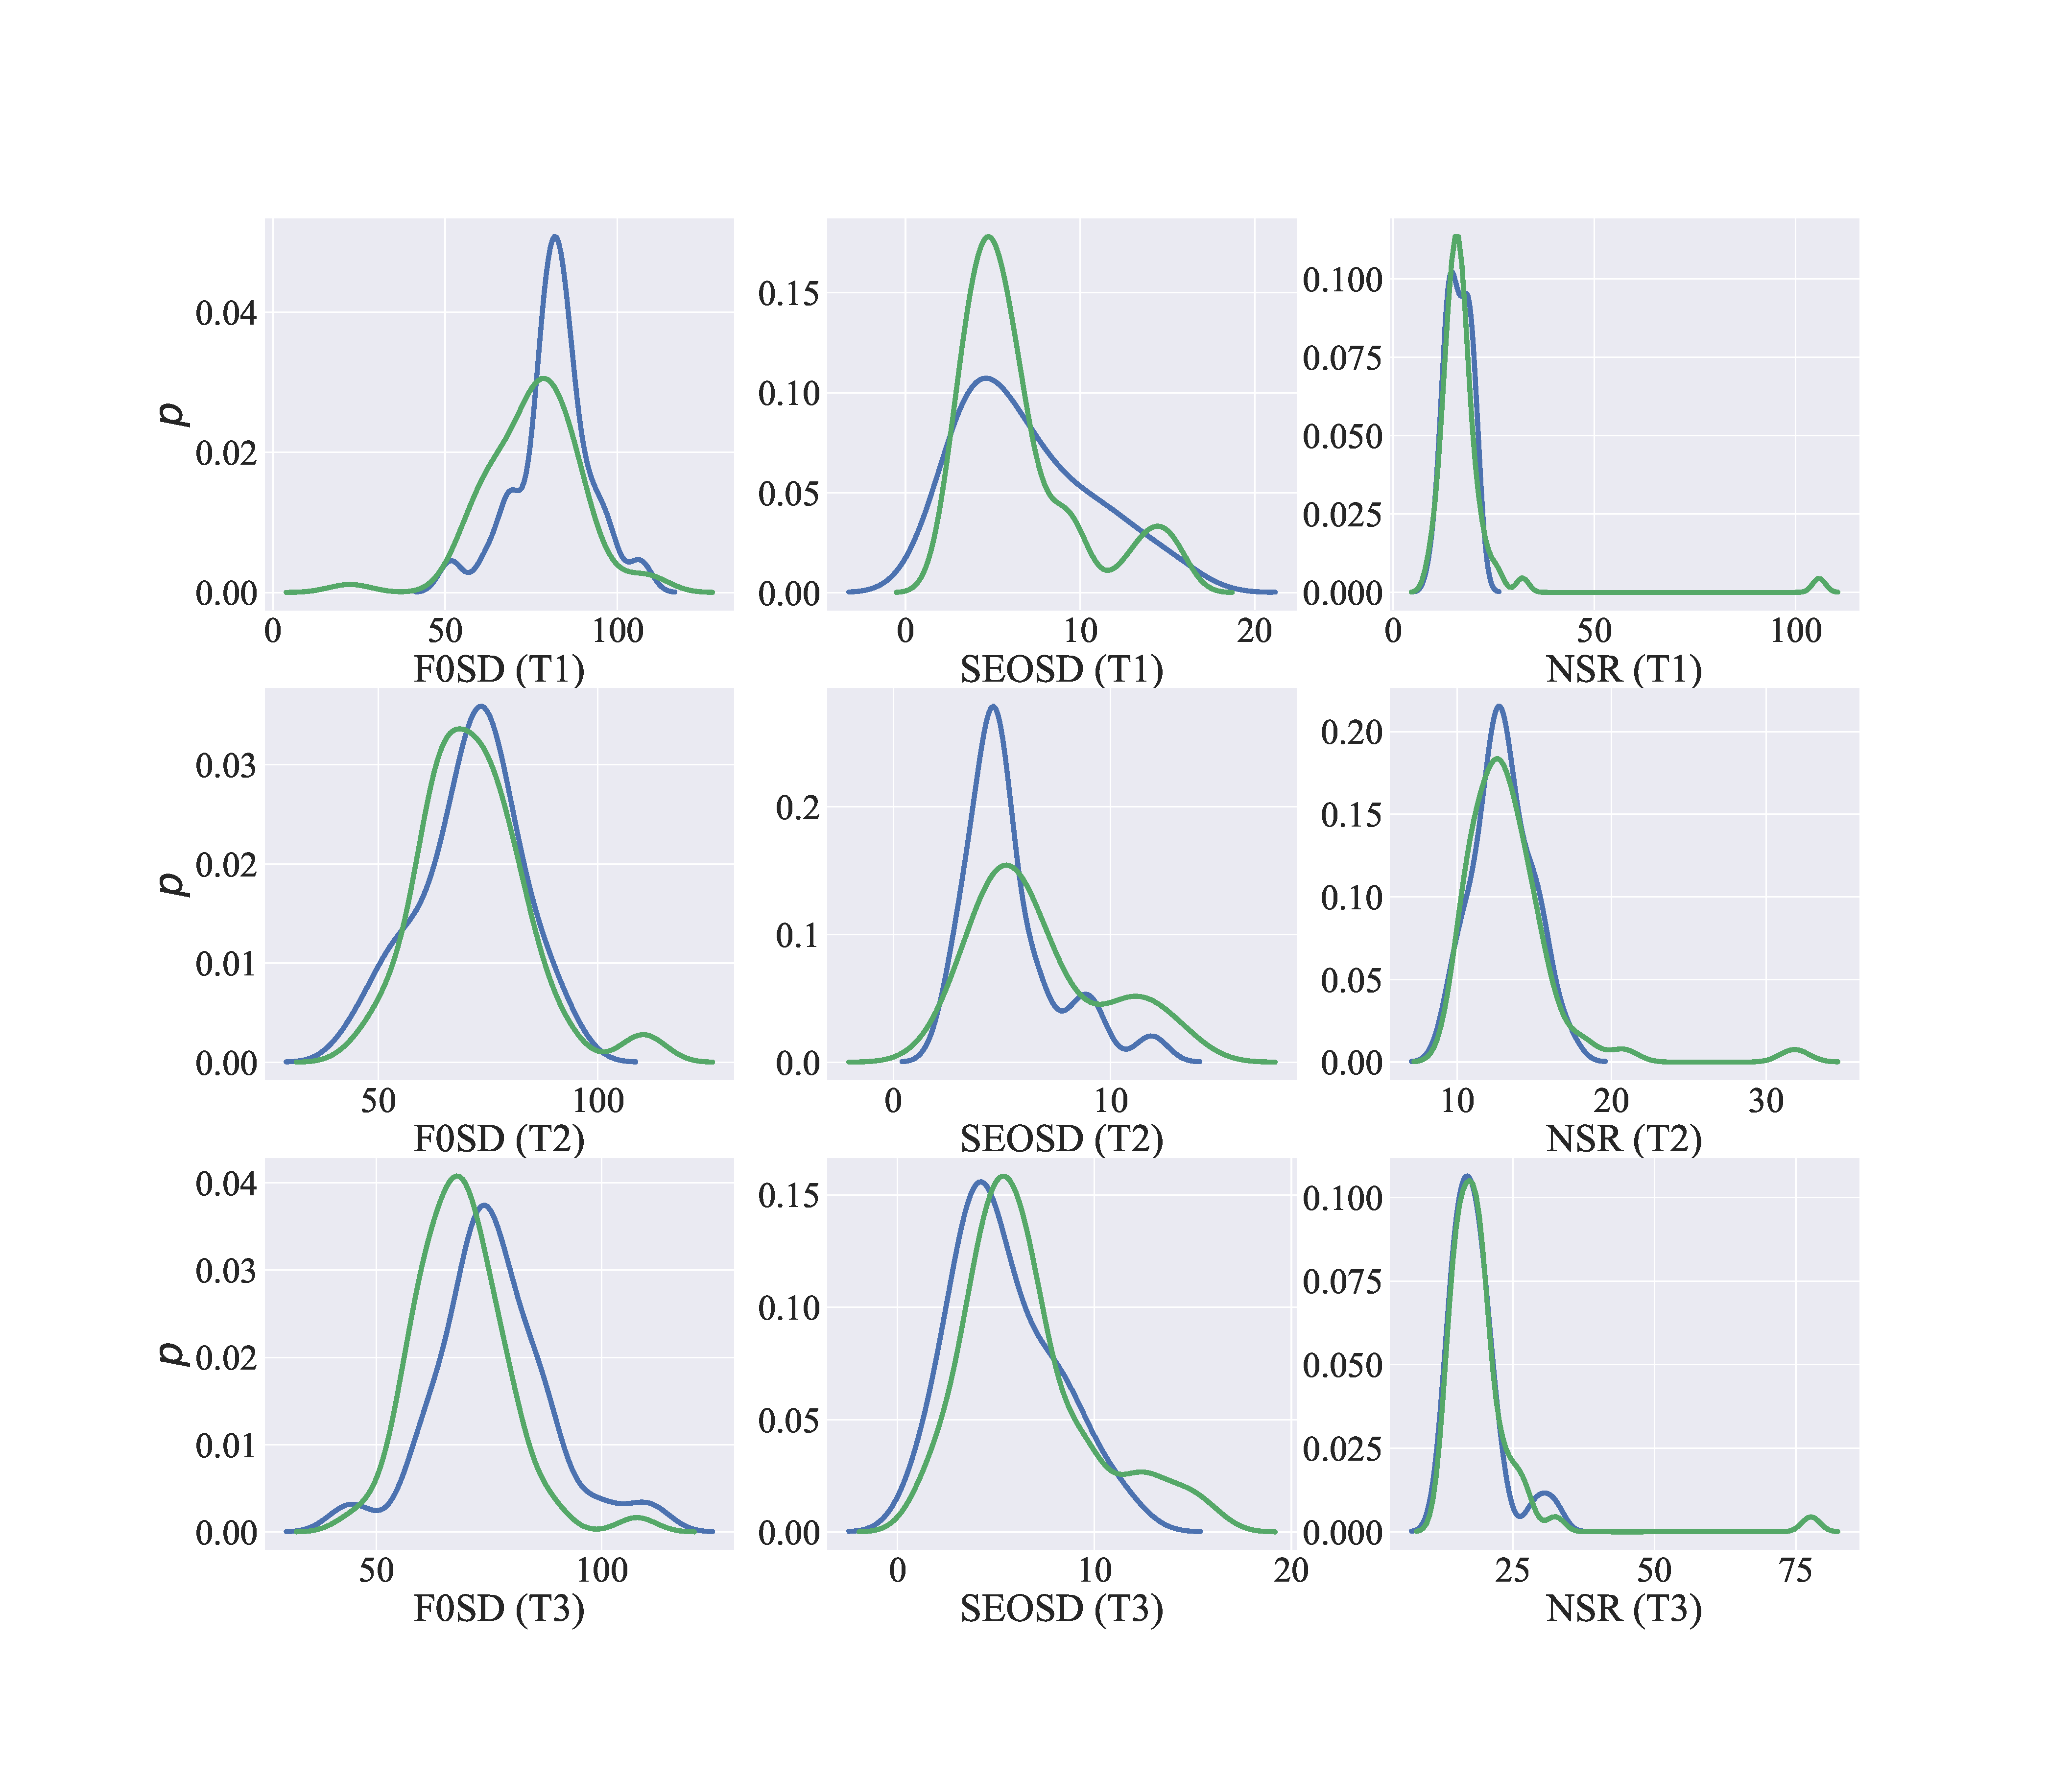
\includegraphics[width=0.99\textwidth]{pictures/ch4_comparisons_males.eps}
	\caption[Density estimation plots for male speakers.]{Density estimation plots (computed using kernel probability density estimation with Gaussian kernels) for selected acoustic features for all three speech tasks performed by male speakers only: T1\,--\,poem recitation task (first row); T2\,--\,emotionally-neutral reading (second row); and T3\,--\,stress-modified reading (third row). Colour notation: blue colour represents healthy speakers, and green colour represents speakers with PD. Feature notation: F0SD (standard deviation of fundamental frequency) expresses variability of intonation (melody of speech); SEOSD (standard deviation of squared energy operator) expresses variability of speech intensity (melody of speech); and NSR (net speech rate) expresses the number of phones per entire duration of speech without pauses (speech rate).}
	\label{fig:ch4_comparisons_males}
\end{figure}

\begin{figure}[htb!]
	\centering
	\scriptsize
	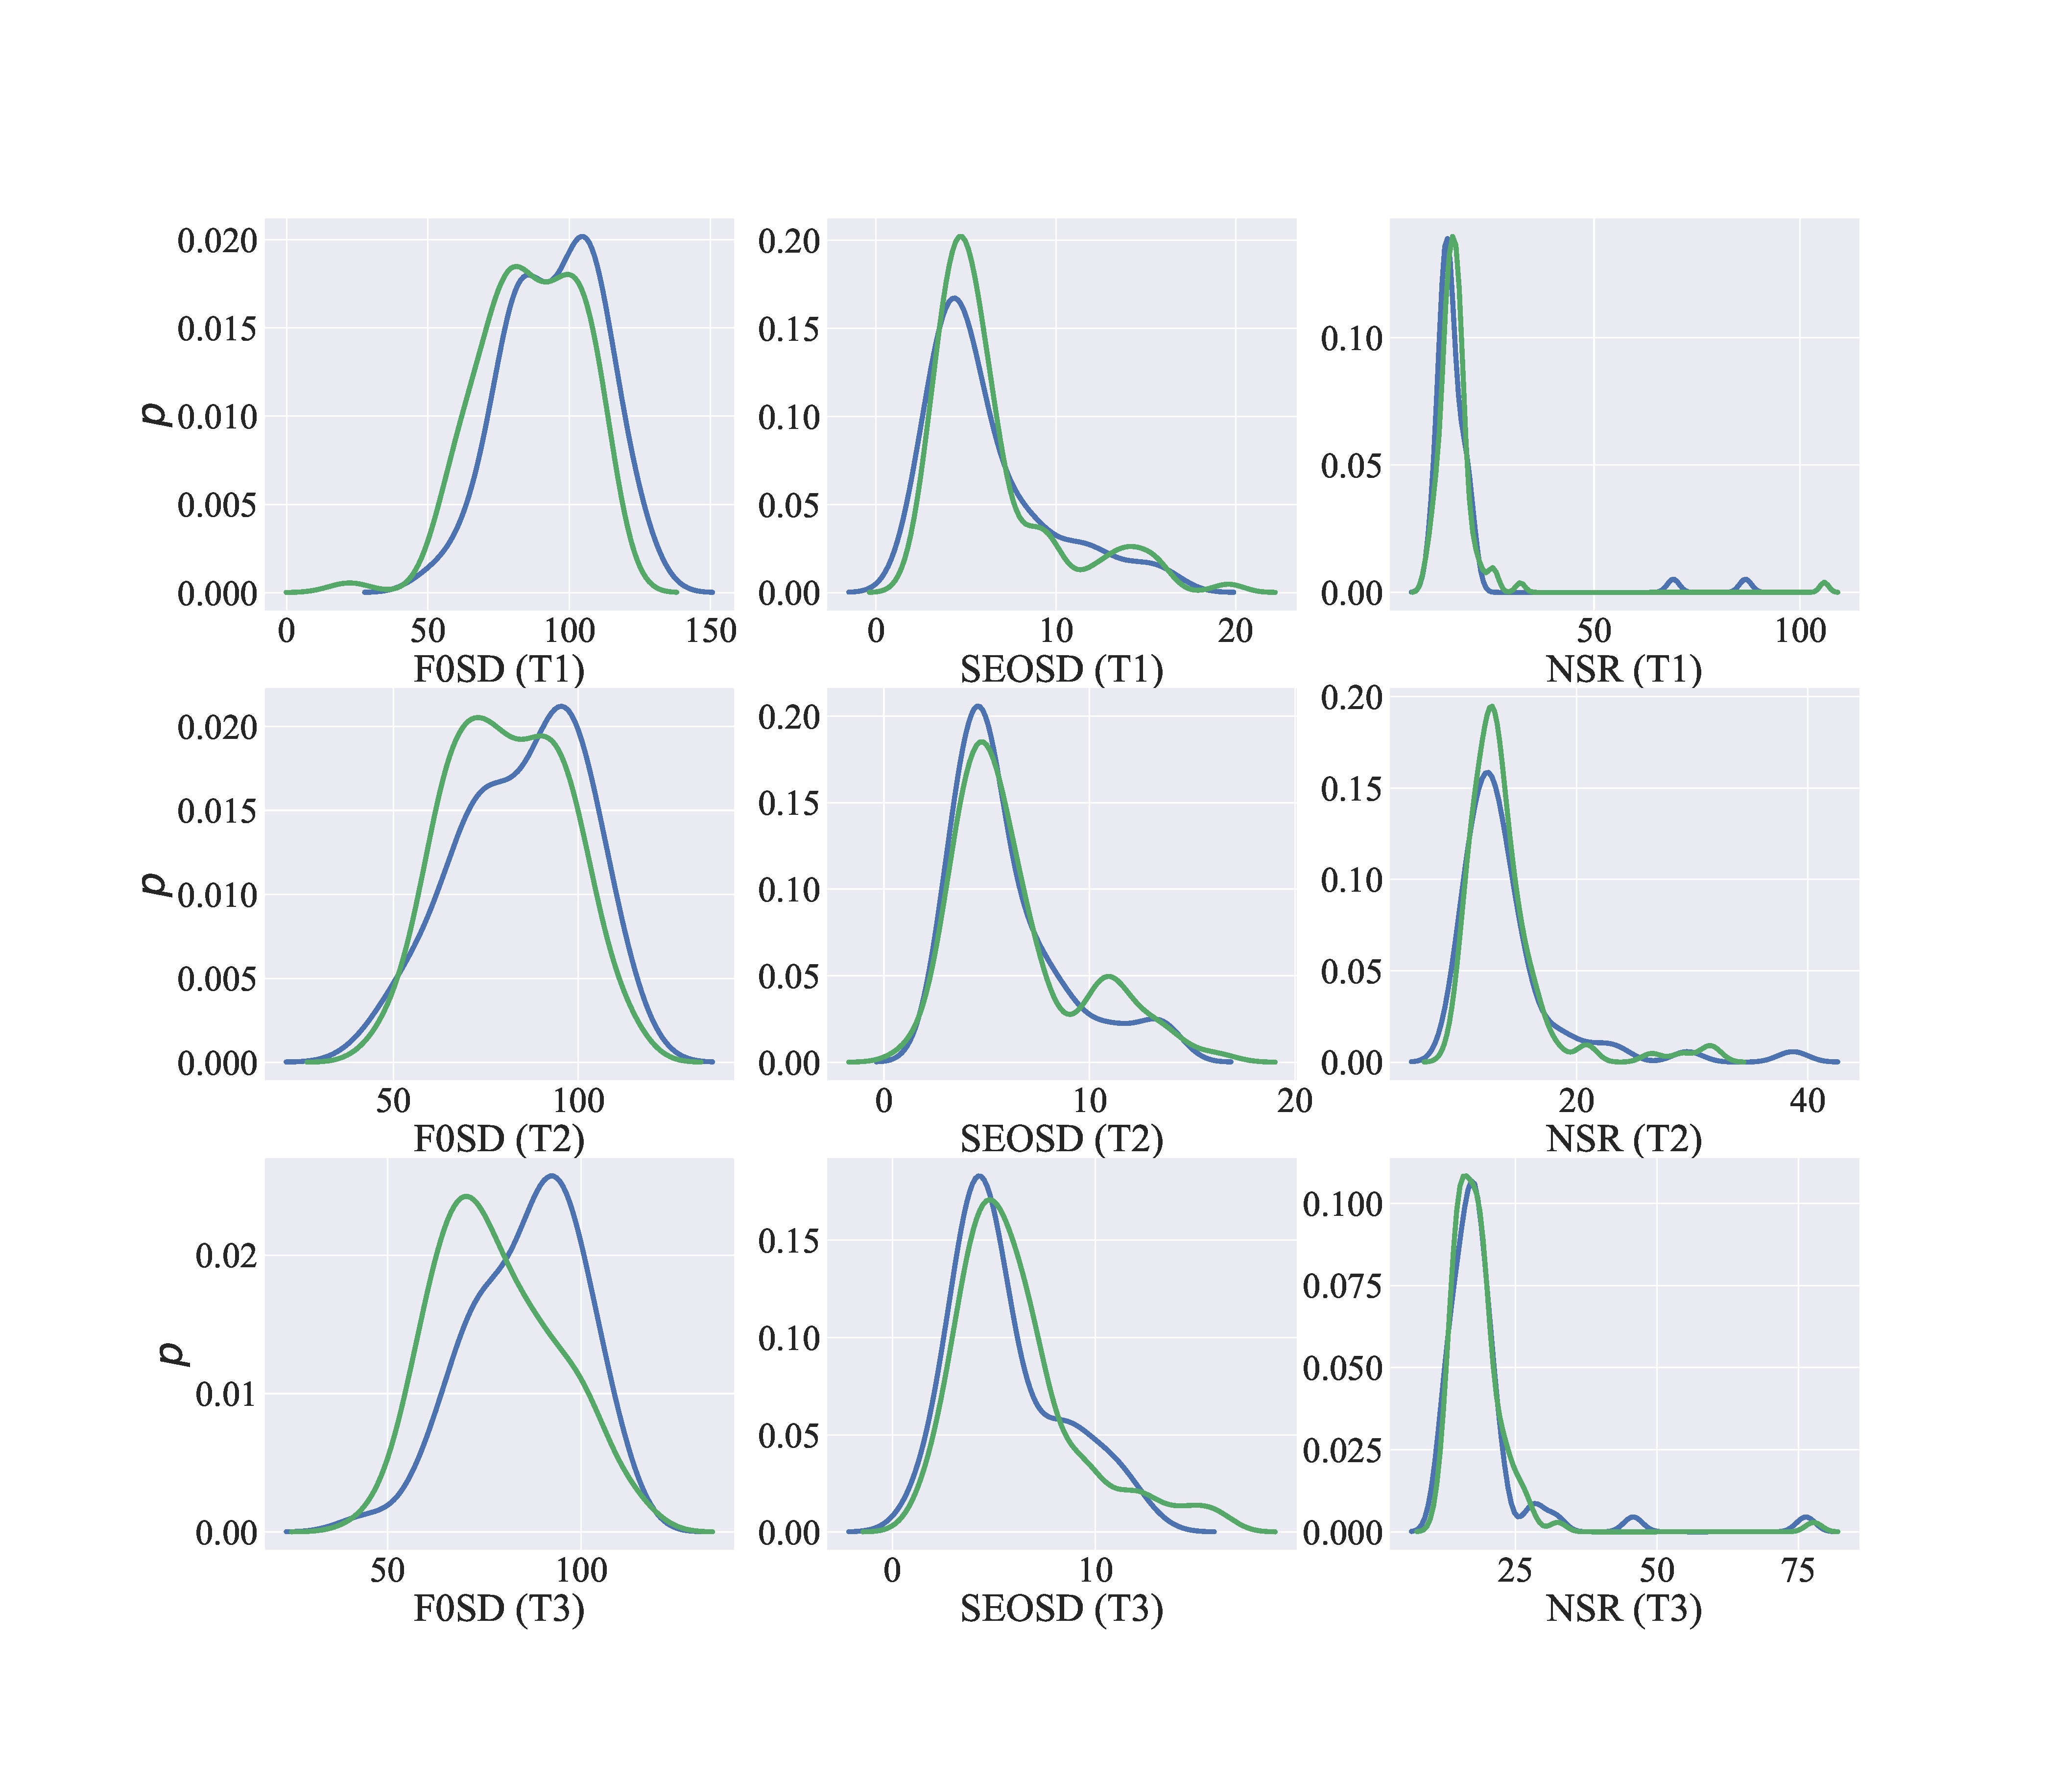
\includegraphics[width=0.99\textwidth]{pictures/ch4_comparisons_all.eps}
	\caption[Density estimation plots for all speakers.]{Density estimation plots (computed using kernel probability density estimation with Gaussian kernels) for selected acoustic features for all three speech tasks performed by all speakers (both genders combined): T1\,--\,poem recitation task (first row); T2\,--\,emotionally-neutral reading (second row); and T3\,--\,stress-modified reading (third row). Colour notation: blue colour represents healthy speakers, and green colour represents speakers with PD. Feature notation: F0SD (standard deviation of fundamental frequency) expresses variability of intonation (melody of speech); SEOSD (standard deviation of squared energy operator) expresses variability of speech intensity (melody of speech); and NSR (net speech rate) expresses the number of phones per entire duration of speech without pauses (speech rate).}
	\label{fig:ch4_comparisons_all}
\end{figure}

As can be seen in Table~\ref{tab:ch4_statistical_analysis}, when the extracted prosodic features are taken individually, the resulting classification performance of the trained models does not reach satisfactory level of accuracy. However, this is somewhat expected since dysprosody in HD is rarely expressed as manifestation in a~single prosodic domain. It is rather a~combination of monopitch, monoloudness and abnormalities in speech rate and pausing. And moreover, HD is also known to be manifested slightly differently from patient to patient, which makes the prediction task even more difficult. Nevertheless, the univariate models can at least provide an indication about the contribution of each of the selected acoustic features to discrimination of dysarthric and healthy speech. So, taking the previously mentioned facts into account, a~feature selection procedure was applied as the next step towards obtaining a~parsimonious, information-rich subsets of features, which provide maximum clinical information about the underlying prosodic pathology in patients with PD. Subsequently, the multivariate models were built using the selected features. The classification performance of these models can be seen in Table~\ref{tab:ch4_classification_groups}, and Table~\ref{tab:ch4_classification_combination}, respectively.

Consequently, t-distributed stochastic neighbourhood embedding (t-SNE)~\cite{Maaten2008} algorithm was used to visualize the multi-dimensional space of prosodic features in the two-dimensional one. For this purpose, all the extracted acoustic features were used. The visualization was performed for all the three speech tasks separately to show the clusters of healthy and dysarthric speakers when speech prosody is quantified in a~robust way (i.\,e. monopitch, monoloudness, and speech rate/pausing abnormalities are described altogether). This method was also applied for female speakers, male speakers, and all speakers (both genders combined). The results of this method are presented in Figure~\ref{fig:ch4_tsne}. As can be seen, using the prosodic description it is not strong enough to conclusively and definitely identify HD in patients with PD. It is important to stress the fact that the results are strongly related to the dataset used in this study. This claim is therefore based on the limited number of samples and must be considered as an approximation of the reality.

\begin{table*}[htb!]
	\centering
	\begin{threeparttable}
		\caption{Classification results for groups of acoustic features.}
		\label{tab:ch4_classification_groups}
		\footnotesize
		\centering
		\begin{tabular}{c l c c c c c c} 
			
			\hline\hline\noalign{\smallskip}
			\rowcolor{gray_table}
			feat. & gender & MCC & ACC & SEN & SPE & $p$ & No. \\
			\noalign{\smallskip}
			\multicolumn{8}{c}{Poem recitation} \\
			\noalign{\smallskip}\hline\noalign{\smallskip}
			
			% Monopitch model
			\multirow{3}{*}{F1} &
			  females & 0.14~$\pm$~0.38 & 58.04~$\pm$~17.71 & 63.00~$\pm$~25.87 & 50.33~$\pm$~32.73 & 0.0910 & 3 \\
			& males   & 0.19~$\pm$~0.39 & 58.15~$\pm$~19.01 & 57.06~$\pm$~24.90 & 61.00~$\pm$~33.94 & 0.0840 & 1 \\
			& all     & 0.17~$\pm$~0.26 & 59.33~$\pm$~12.43 & 61.35~$\pm$~14.68 & 55.53~$\pm$~21.15 & 0.1690 & 1 \\
			\noalign{\smallskip}
			
			% Monoloudness model
			\multirow{3}{*}{F2} &
			  females & 0.24~$\pm$~0.40 & 61.28~$\pm$~18.47 & 59.50~$\pm$~27.14 & 63.66~$\pm$~28.70 & 0.2590 & 8 \\
			& males   & 0.26~$\pm$~0.41 & 65.93~$\pm$~17.78 & 72.06~$\pm$~20.38 & 53.33~$\pm$~34.17 & 0.0090 & 6 \\
			& all     & 0.23~$\pm$~0.27 & 62.78~$\pm$~12.58 & 66.24~$\pm$~16.70 & 56.40~$\pm$~25.64 & 0.0020 & 3 \\
			\noalign{\smallskip}
			
			% Speech rate model
			\multirow{3}{*}{F3} &
			  females & 0.19~$\pm$~0.43 & 59.28~$\pm$~20.25 & 60.00~$\pm$~27.66 & 58.66~$\pm$~30.53 & 0.0790 & 2 \\
			& males   & 0.29~$\pm$~0.42 & 63.49~$\pm$~20.05 & 61.73~$\pm$~24.04 & 67.66~$\pm$~32.54 & 0.0130 & 1 \\
			& all     & 0.27~$\pm$~0.24 & 64.02~$\pm$~11.35 & 65.80~$\pm$~19.08 & 61.00~$\pm$~24.55 & 0.0010 & 1 \\
			\noalign{\smallskip}
			
			\noalign{\smallskip}\hline\noalign{\smallskip}
			\multicolumn{8}{c}{Reading with neutral emotion} \\
			\noalign{\smallskip}\hline\noalign{\smallskip}
			
			% Monopitch model
			\multirow{3}{*}{F1} &
			  females & 0.13~$\pm$~0.42 & 54.85~$\pm$~19.35 & 49.50~$\pm$~28.34 & 63.33~$\pm$~31.22 & 0.1450 & 3 \\
			& males   & 0.11~$\pm$~0.33 & 59.39~$\pm$~13.56 & 65.60~$\pm$~17.45 & 45.33~$\pm$~32.12 & 0.1340 & 2 \\
			& all     & 0.08~$\pm$~0.24 & 54.67~$\pm$~11.19 & 56.68~$\pm$~17.85 & 50.86~$\pm$~24.79 & 0.5910 & 3 \\
			\noalign{\smallskip}
			
			% Monoloudness model
			\multirow{3}{*}{F2} &
			  females & 0.16~$\pm$~0.44 & 58.19~$\pm$~20.29 & 59.50~$\pm$~28.07 & 56.00~$\pm$~31.90 & 0.1590 & 3 \\
			& males   & 0.37~$\pm$~0.42 & 70.53~$\pm$~19.62 & 74.60~$\pm$~20.34 & 62.33~$\pm$~30.64 & 0.0080 & 4 \\
			& all     & 0.19~$\pm$~0.28 & 60.90~$\pm$~13.00 & 63.97~$\pm$~15.55 & 55.33~$\pm$~23.27 & 0.1420 & 3 \\
			\noalign{\smallskip}
			
			% Speech rate model
			\multirow{3}{*}{F3} &
			  females & 0.30~$\pm$~0.37 & 64.04~$\pm$~17.63 & 65.00~$\pm$~25.25 & 62.66~$\pm$~29.84 & 0.0510 & 2 \\
			& males   & 0.20~$\pm$~0.31 & 60.31~$\pm$~15.40 & 61.73~$\pm$~20.89 & 58.00~$\pm$~26.98 & 0.0710 & 1 \\
			& all     & 0.12~$\pm$~0.30 & 56.17~$\pm$~13.89 & 56.53~$\pm$~15.02 & 55.80~$\pm$~23.82 & 0.3260 & 4 \\
			\noalign{\smallskip}
			
			\noalign{\smallskip}\hline\noalign{\smallskip}
			\multicolumn{8}{c}{Stress-modified reading} \\
			\noalign{\smallskip}\hline\noalign{\smallskip}
			
			% Monopitch model
			\multirow{3}{*}{F1} &
			  females & 0.31~$\pm$~0.35 & 64.38~$\pm$~15.63 & 67.50~$\pm$~25.87 & 60.33~$\pm$~30.84 & 0.0990 & 2 \\
			& males   & 0.21~$\pm$~0.38 & 61.74~$\pm$~17.71 & 63.80~$\pm$~21.02 & 57.66~$\pm$~31.26 & 0.1280 & 2 \\
			& all     & 0.15~$\pm$~0.26 & 58.37~$\pm$~13.13 & 61.60~$\pm$~17.21 & 52.73~$\pm$~19.60 & 0.1560 & 2 \\
			\noalign{\smallskip}
			
			% Monoloudness model
			\multirow{3}{*}{F2} &
			  females & 0.40~$\pm$~0.26 & 69.66~$\pm$~12.01 & 72.00~$\pm$~21.21 & 65.66~$\pm$~26.60 & 0.0240 & 3 \\
			& males   & 0.24~$\pm$~0.41 & 63.30~$\pm$~18.24 & 64.73~$\pm$~20.68 & 59.66~$\pm$~33.51 & 0.0360 & 4 \\
			& all     & 0.20~$\pm$~0.21 & 61.95~$\pm$~9.15  & 66.35~$\pm$~13.55 & 53.86~$\pm$~21.57 & 0.1150 & 2 \\
			\noalign{\smallskip}
			
			% Speech rate model
			\multirow{3}{*}{F3} &
			  females & 0.15~$\pm$~0.39 & 58.90~$\pm$~15.39 & 63.50~$\pm$~19.69 & 51.66~$\pm$~35.99 & 0.4570 & 2 \\
			& males   & 0.24~$\pm$~0.32 & 64.44~$\pm$~14.19 & 68.73~$\pm$~18.64 & 55.66~$\pm$~30.41 & 0.0650 & 1 \\
			& all     & 0.13~$\pm$~0.25 & 58.15~$\pm$~12.36 & 62.02~$\pm$~17.18 & 51.13~$\pm$~21.88 & 0.6840 & 2 \\
			\noalign{\smallskip}
			
			\noalign{\smallskip}\hline\hline
		\end{tabular}
		
		\begin{tablenotes}
			\scriptsize
			\item Table notation: F1\,--\,monopitch features; F2\,--\,monoloudness features; F3\,--\,speech rate features; F4\,--\,general prosodic features; MCC\,--\,Matthew's correlation coefficient (dimensionless)~\cite{Matthews1975}; ACC\,--\,classification accuracy (expressed in $\%$); SEN\,--\,classification sensitivity (expressed in $\%$); SPE\,--\,classification specificity (expressed in $\%$); No.\,--\,number of selected features; $p$\,--\,p-values of classification calculated by permutation test ($1000$ permutations).
		\end{tablenotes}
	\end{threeparttable}
\end{table*}

\begin{table*}[htb!]
	\centering
	\begin{threeparttable}
		\caption{Classification results for all acoustic features.}
		\label{tab:ch4_classification_combination}
		\footnotesize
		\centering
		\begin{tabular}{c l c c c c c c} 
		
			\hline\hline\noalign{\smallskip}
			\rowcolor{gray_table}
			feat. & gender & MCC & ACC & SEN & SPE & $p$ & No. \\
			\noalign{\smallskip}\hline\noalign{\smallskip}

			\multirow{3}{*}{T1} &
			  females & 0.36~$\pm$~0.42 & 66.57~$\pm$~19.80 & 66.00~$\pm$~25.13 & 68.33~$\pm$~30.90 & 0.0070 & 5 \\
			& males   & 0.35~$\pm$~0.34 & 67.84~$\pm$~17.33 & 68.93~$\pm$~22.54 & 66.00~$\pm$~27.34 & 0.0020 & 3 \\
			& all     & 0.33~$\pm$~0.16 & 67.30~$\pm$~08.42 & 68.84~$\pm$~14.18 & 64.66~$\pm$~14.98 & 0.0040 & 1 \\
			\noalign{\smallskip}

			\multirow{3}{*}{T2} &
			  females & 0.37~$\pm$~0.40 & 68.47~$\pm$~18.64 & 72.00~$\pm$~26.06 & 63.33~$\pm$~31.94 & 0.2110 & 3 \\
			& males   & 0.38~$\pm$~0.29 & 69.52~$\pm$~14.02 & 70.40~$\pm$~18.93 & 68.00~$\pm$~26.90 & 0.0050 & 8 \\
			& all     & 0.16~$\pm$~0.32 & 59.62~$\pm$~15.80 & 64.93~$\pm$~18.77 & 50.13~$\pm$~21.36 & 0.0350 & 4 \\
			\noalign{\smallskip}

			\multirow{3}{*}{T3} &
			  females & 0.42~$\pm$~0.35 & 70.71~$\pm$~16.24 & 71.00~$\pm$~19.13 & 70.33~$\pm$~30.91 & 0.0001 & 1 \\
			& males   & 0.37~$\pm$~0.34 & 70.03~$\pm$~16.05 & 73.53~$\pm$~19.28 & 63.00~$\pm$~29.41 & 0.0120 & 5 \\
			& all     & 0.25~$\pm$~0.26 & 63.20~$\pm$~12.44 & 65.06~$\pm$~14.92 & 60.00~$\pm$~21.07 & 0.0130 & 3 \\	

			\noalign{\smallskip}\hline\hline
		\end{tabular}
				
		\begin{tablenotes}
			\scriptsize
			\item Table notation: T1\,--\,poem recitation task; T2\,--\,reading with neutral emotion; T3\,--\,stress-modified reading task; MCC\,--\,Matthew's correlation coefficient (dimensionless)~\cite{Matthews1975}; ACC\,--\,classification accuracy (expressed in $\%$); SEN\,--\,classification sensitivity (expressed in $\%$); SPE\,--\,classification specificity (expressed in $\%$); No.\,--\,number of selected features; $p$\,--\,p-values of classification calculated by permutation test ($1000$ permutations).
		\end{tablenotes}
	\end{threeparttable}
\end{table*}

\begin{figure}[htb!]
	\centering
	\scriptsize
	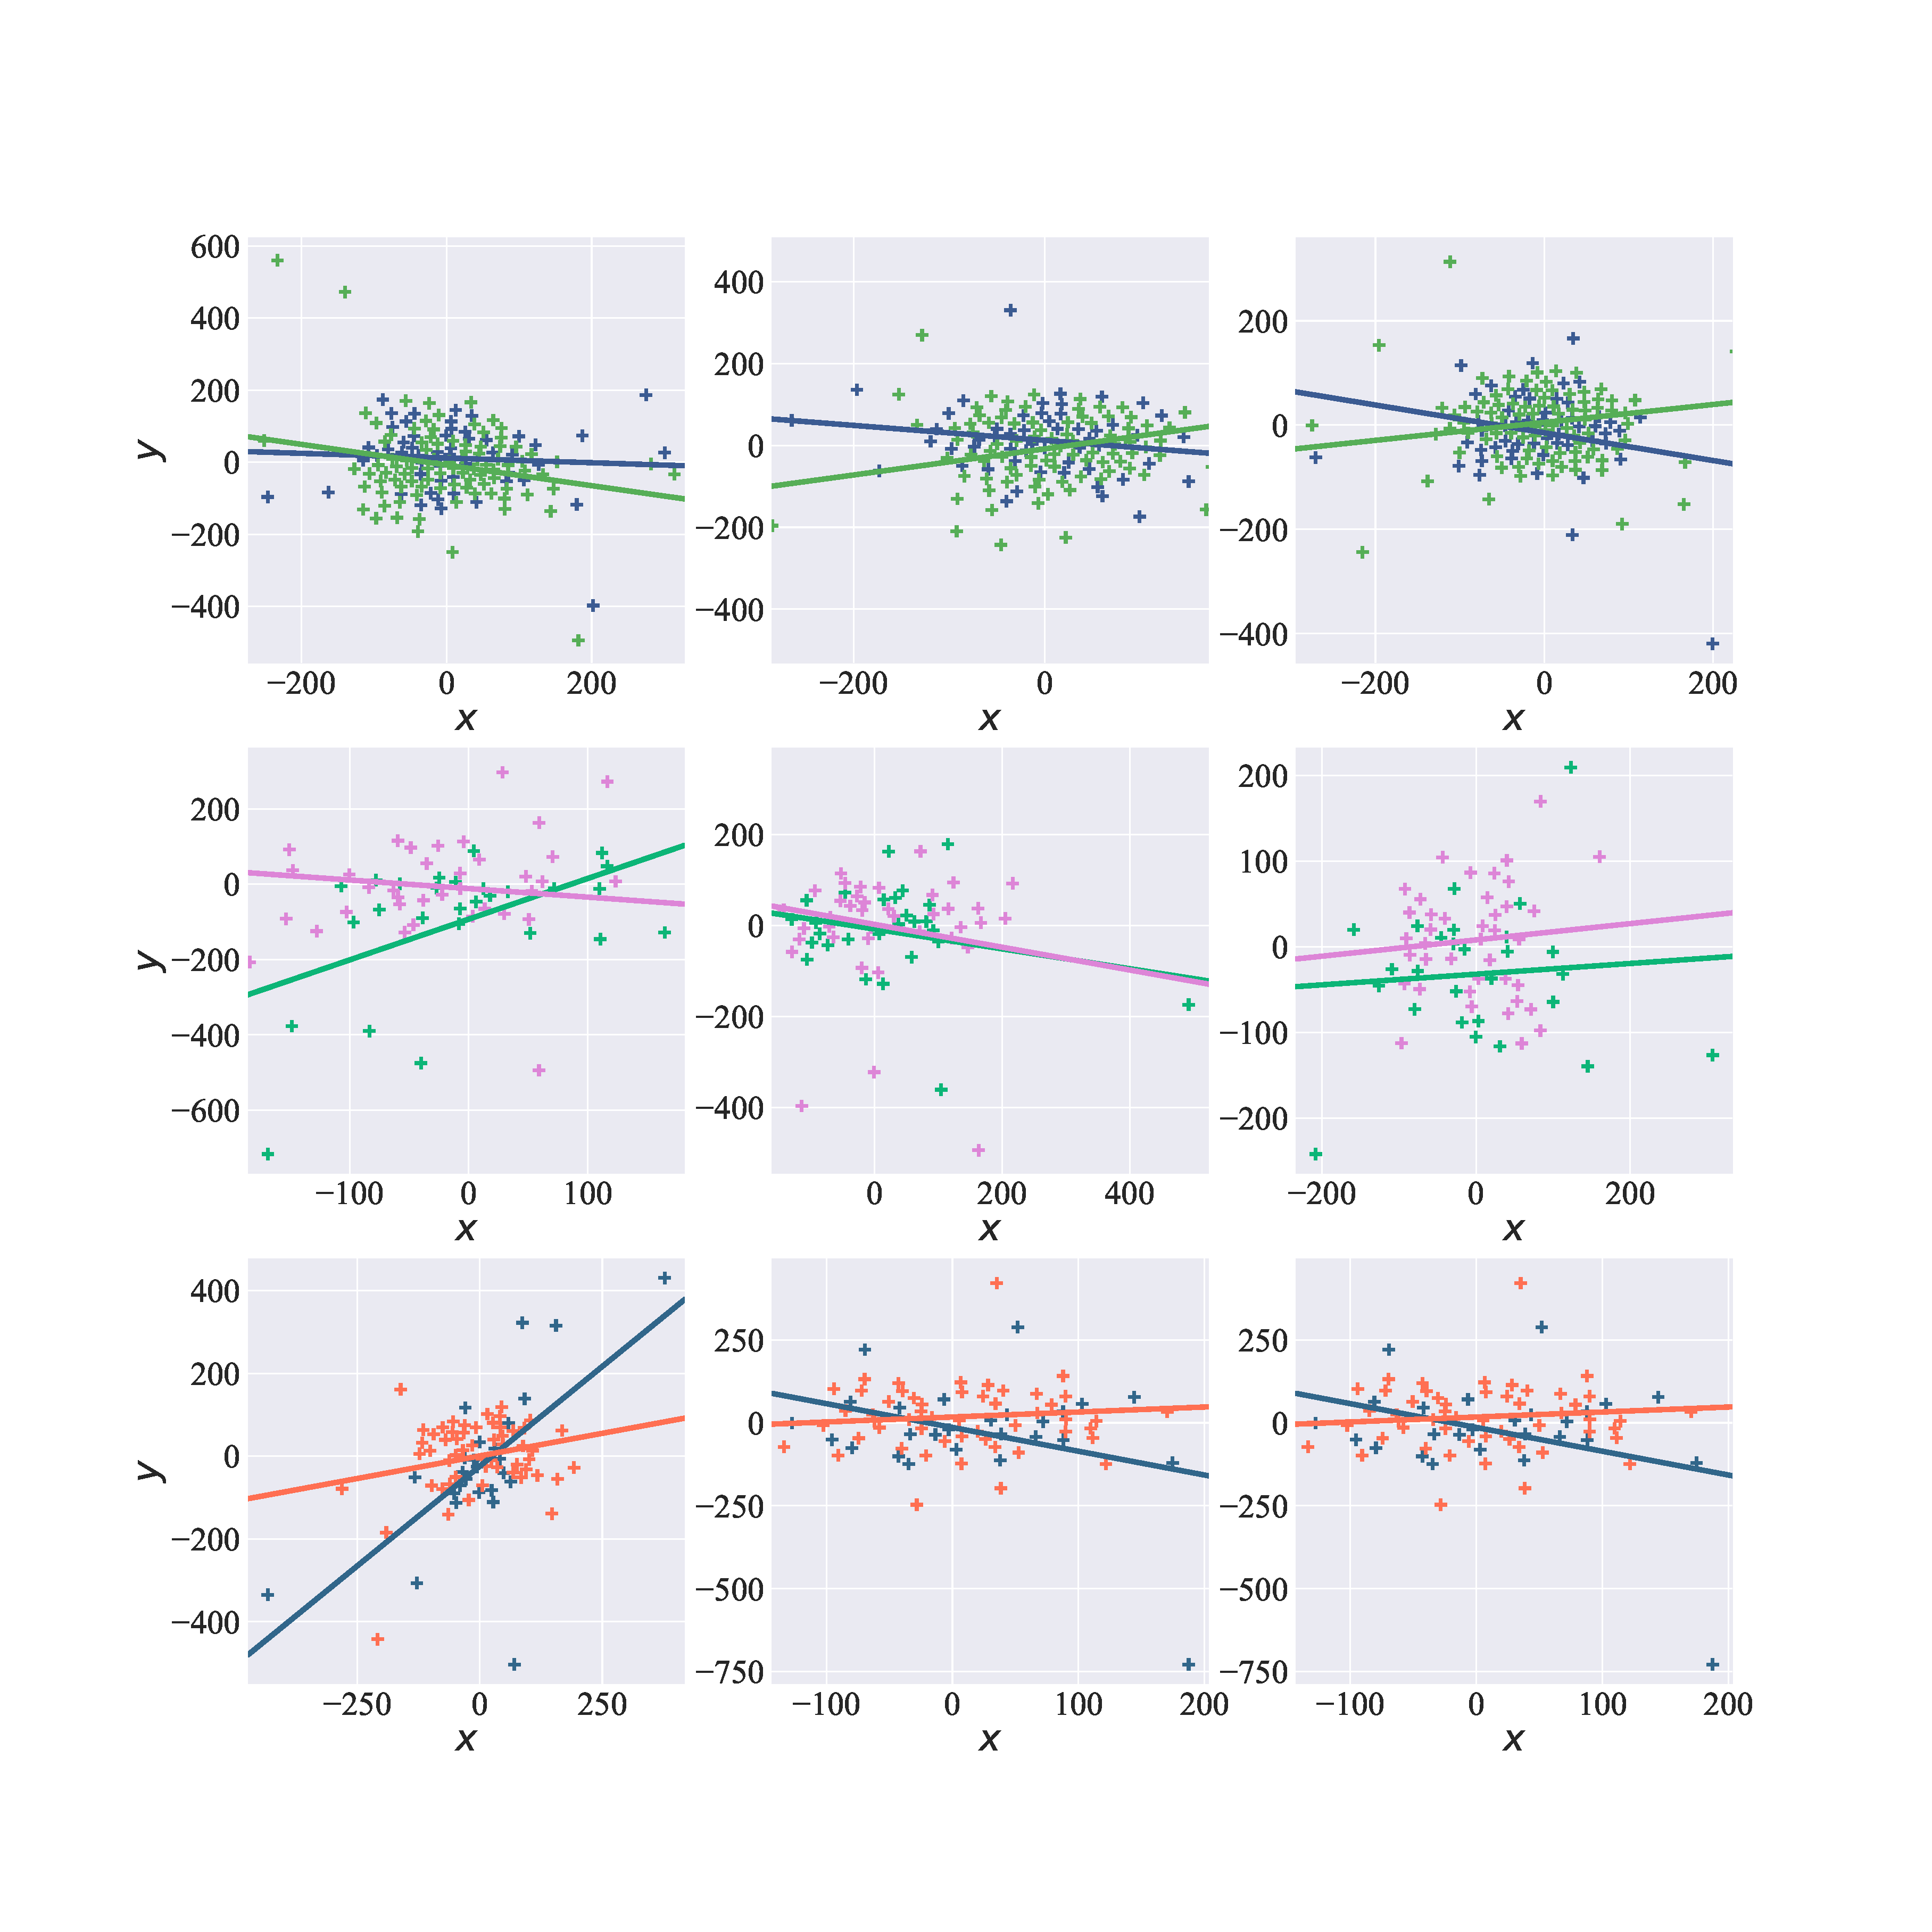
\includegraphics[width=0.99\textwidth]{pictures/ch4_tsne_separated.eps}
	\caption[t-distributed stochastic neighbourhood embedding visualization.]{Visualization of t-distributed stochastic neighbourhood embedding applied on all samples and acoustic features for each of the speech tasks separately (lines fitted using robust linear regression for each visualized class are provided as well). Graph grid notation: $1$. row\,--\,all speakers, $2$. row\,--\,female speakers, $3$. row\,--\,male speakers; $1$. column\,--\,poem recitation task, $2$. column\,--\,emotionally-neutral reading, $3$. column\,--\,stress-modified reading. Colour notation: all speakers\,--\,dark blue colour represents healthy speakers, and dark green colour represents speakers with PD; female speakers\,--\,medium green colour represents healthy speakers, and purple colour represents speakers with PD; and male speakers\,--\,medium blue colour represents healthy speakers, and orange colour represents speakers with PD. Note: the feature space is reduced from multi-dimensional space to two-dimensional one and therefore only general $x$, $y$ features are used to describe the resulting feature space.}
	\label{fig:ch4_tsne}
\end{figure}

\newpage
To specify the results presented in these two tables: Table~\ref{tab:ch4_classification_groups} shows the results of the multivariate classification analysis employed on the subsets of the prosodic features. Specifically, models for monopitch (F1), monoloudness (F2), and speech rate abnormalities (F3) were built. The assumption behind this approach was that despite insufficiency of the univariate models, investigation of the classification performance of each of the prosodic manifestations in HD can improve the performance of the models when more features are being used (it needs to be pointed out that these features do however describe the same phenomenon so that they are quiet correlated. But as mentioned previously, RF classifier is robust in dealing with high-dimensional and highly correlated data). Table~\ref{tab:ch4_classification_combination} shows the results of the multivariate classification analysis employed on all of the prosodic features (F4).

The best classification performance in terms of classification accuracy achieved using the prosodic features for each speech task separately can be summarized as follows: a) poem recitation task\,--\,$\mbox{ACC}=67.84\,\%$ the model was trained using only $3$ features based on the analysis of general prosodic impairment (TPT, TEOSD, SEOSD) computed for male participants; b) reading with neutral emotion\,--\,$\mbox{ACC}=69.52\,\%$, the model was trained using $8$ features based based on the analysis of general prosodic impairment (SEOSD, relF0SD, TST, TPT, relSEOSD, TPT\,(50\,ms), relSEOVR, NSR) computed for male participants; and finally c) stress-modified reading\,--\,$\mbox{ACC}=70.71\,\%$, the model was trained using just a~single feature based on the analysis of monoloudness (relTEOVR) computed for female participants. It is worth noting that some of these models did not achieve sufficiently low p-values of the permutation test (strict significance level of $0.01$ was chosen) that is needed to reject the null hypothesis. This may indicated that more data are required in order to get significant results~\cite{Golland2005}.

With respect to the models built for the subsets of the prosodic features and all of the features taken together (general prosodic model), the following classification performance was achieved: F1\,--\,$\mbox{ACC}=64.38\,\%$, the model was trained using prosodic features extracted from the stress-modified reading task performed by female participants; F2\,--\,$\mbox{ACC}=70.54\,\%$, the model was trained using prosodic features extracted from the reading task with neutral emotion performed by male participants; F3\,--\,$\mbox{ACC}=64.44\,\%$, the model was trained using prosodic features extracted from the stress-modified reading task performed by male participants; and finally F4\,--\,$\mbox{ACC}=70.71\,\%$, the model was trained using prosodic features extracted from the stress-modified reading task performed by male participants.

\section{Conclusion}
\label{ch4_5}

According to the literature \cite{Ho1998, Goberman2005d}, speech task used for the assessment of voice and speech has a~great impact on the prosodic aspects of HD. Moreover, as stated by Skodda et al. in $2011$, some aspects of prosody might be different in natural conversational speech in comparison to other speech tasks. Thus, in the frame of this study, three types of speech tasks are used: a) reading with neutral emotion\,--\,to obtain data comparable with previous studies \cite{Skodda2008, Skodda2010, Skodda2011c, Rusz2011} that also used speech tasks focusing on reading with neutral emotion in their analysis setup. To some extent the results are also comparable with the work of Bandini et al.~\cite{Bandini2015} that focused on the automatic identification of dysprosody in HD using a~sentence repetition task; b) stress-modified reading\,--\,to obtain data that are at least partially comparable with those proposed in the research of Tykalova et al.~\cite{Tykalova2014} focused on the acoustic investigation of stress patterns in PD using a~reading task. But the main idea behind this approach was to expose speakers to additional prosodic demands, which in theory could emphasize the prosodic impairment in the group of PD patients as opposed to the HC.

Regarding the individual analysis of the selected acoustic features quantifying dysprosody in HD, the following conclusion can be made. At first, this study confirms previous finding of several renowned researchers \cite{Canter1965, Metter1986, Flint1992, Goberman2005b, Skodda2011c} reporting that patients with PD exhibit decreased intonation variability in comparison with HC (difference of approximately $8.72\,\%$). This pattern can be seen in almost every scenario used in this study except a~single reading task performed by the male participants with neutral emotion. This suggests that emotionally-neutral reading, especially in the male subjects is not sufficient enough to capture monopitch. In contrast, speech tasks such as stress-modified reading and a~recitation task seems to be a~good candidates for further investigation. Interestingly, at the same time, the results suggests that PD patients produce higher variability in speech intensity than HC (difference of approximately $12.41\,\%$), which is in contradiction with the previous findings published in \cite{Metter1986, Watson2008, Rusz2011, Skodda2011c}. However, this might be a~consequence of a~presence of so far uncovered gender-related pattern of speech intensity control impairment in HD, especially in the dataset used in the frame of this study, which is based on the observation of great gender-related distinctions of speech intensity deterioration summarized in Table~\ref{tab:ch4_comparisons}. Therefore, subsequent investigation of this phenomenon would be of interest. And finally, concerning speech rate abnormalities, the results suggest that PD patients in general produce lower speech rate that HC when performing a~task that requires prosodic demands such as stress or melody alternation. Regarding the gender-related distinctions, male participants seem to have have higher speech rate when compared to HC. Nevertheless, this is likely a~dataset-specific pattern that would need to be confirmed using a~different and possibly multilingual dataset.

Next, with respect to the comparison between emotionally-neutral and stress-modified reading. The following conclusion can be drawn: the classification accuracy achieved for the model based on the stress-modified reading performed by female speakers ($70.71\,\%$) and the model based on the emotionally-neutral reading performed by male speakers ($69.52\,\%$), may indicate no difference between these two tasks. However, deeper investigation considerably favours the stress-modified reading tasks considerably. The main reasons supporting this conclusion are: a) the p-value computed using permutation test is significantly lower in the case of stress-modified reading ($p=0.0001$) in contrast with the emotionally-neutral one ($p=0.0050$) suggesting higher reliability and statistical significance of the results; b) when the feature selection was applied, only a~single prosodic feature (relTEOVR) expressing monoloudness was needed to provide sufficient power to discriminate dysarthric and healthy speech, whereas eight features were selected in the case of emotionally-neutral reading task. Therefore, the clinical interpretability of the results derived from the reading with stress emphasis is far more convenient and practical. One more important aspect to consider is the fact that the two results also differ in their corresponding gender group. Nevertheless, in the case of emotionally-neutral reading, the results achieved for the group of female speakers are comparable to the ones achieved for the male group. Moreover, the statistical significance of this case was rejected anyway.

With respect to the comparison between the poem recitation task and the reading tasks, the results shows that the poem recitation task outperformed both reading tasks in the case of gender-undifferentiated analysis. This suggests that recitation-related rhythmical demands can in general lead to more precise discrimination of dysprosody in HD in cases when gender-differentiation is not required. In contrast to the straightforwardness of this outcome, the gender information consideration inflicted higher classification accuracy of stress-modifier reading compared to the poem recitation. One can hypothesize this may be a~consequence of some yet to be found gender-related pattern of rhythm and stress control deterioration present in HD. Furthermore, it is also important to emphasize the difference in gender group sizes (the mixed group contains approximately twice as many speakers than the gender-separated groups), therefore the difference in performance could be caused by an independent phenomena. Nevertheless, this hypothesis needs to be confirmed by the subsequent investigation. Another interesting observation made here is the striking proximity of the classification accuracies achieved by the emotionally-neutral reading and the poem recitation. Considering that when no prosodic demands such as rhythm, stress or emotion are required, marked superiority of the poem recitation would be naturally anticipated. Nevertheless, permutation test repeatedly gave disadvantage to the results achieved for the reading with neutral emotion.

Finally, When discriminating dysarthric and healthy speech using several scenarios focused on the expression of monopitch, monoloudness, speech rate abnormalities and a~combination of these prosodic flaws, the results showed that the analysis of a~single aspect of parkinsonian dysprosody (using this particular set of features) does not achieve sufficient classification accuracy, which is in some respect consistent with the results proposed by Lowit~\cite{Lowit2008} in $2008$ in which the author stated that a~combination of these aspects should be analysed exclusively. As can be seen in Table~\ref{tab:ch4_comparisons} this fact is also supported by the p-values computed using the permutation test that in most cases rejected the hypothesis of statistical significance of these prosodic sub-models. In contrast, the analysis of general prosodic features improved the classification accuracies of the models. Therefore, it can be concluded that future development of novel prosodic features quantifying the relationship between monopitch, monoloudness and speech rate disruption in PD is likely to bring deeper understanding of HD and its manifestation on human speech prosody.

To guarantee a~complete and relevant overview, limitations of this work need to be pointed out. With respect to the speech sample, one drawback (which is a~common one of many studies dealing with the acoustic analysis of speech in PD) is relatively small dataset restricting overall statistical significance of the results. Additionally, since the prevalence rate of PD is estimated to approximately $1.5\,\%$ (for people aged over 65 years, see~\cite{Rijk1997}), investigated data should reflect this fact. However, most dataset comprise more PD patients than healthy speakers, which therefore does not correspond with the reality. This is also the case of this particular work. Moreover, it is also worth noting that the current results are based upon speech tasks of relatively limited length. As suggested by Rusz et al. in~\cite{Rusz2013, Rusz2013b} acoustic features computed from a~running speech are the most prospective ones to assess the speech impairment in PD. So, an addition of the running speech can in general bring new insights into understanding of differences among neutral, stressed, rhymed and spontaneous speech in patients with PD. Finally, no correction of the p-values obtained by the Mann-Whitney U~test and Spearman's correlation was performed. However, since the tests were executed only on carefully selected set of $19$ prosodic features, the errors caused by the multiple testing issue are not as relevant as they could be if hundreds or thousands of features were used.

To summarize, the results confirms the previous findings of reduced pitch variation~\cite{Canter1963, Metter1986, Flint1992, Goberman2005b, Goberman2005d, Rusz2011}, to some extent impaired speech intensity control~\cite{Metter1986, Watson2008, Skodda2011c, Rusz2011, Clark2014} and speech rate abnormalities~\cite{Weismer1984, Metter1986, Skodda2008, Skodda2011c} in PD. The results also highlight the fact that more studies are necessary in order to fully understand the manifestation of HD on human prosody. In $2009$, Skodda et al.~\cite{Skodda2009} used prosodic features to study changes of speech rate and pitch variation in patients with PD over time and showed the presence of some characteristic changes in parkinsonian dysprosody. However, further longitudinal studies are required. Besides the PD classification and disease tracking, the analysis of dysprosody in HD can also be used during an evaluation of the modern non-invasive treatment methods such as high-frequency repetitive transcranial magnetic stimulation (rTMS)~\cite{Eliasova2013}, which has a~great potential in treatment of PD. 